% Options for packages loaded elsewhere
\PassOptionsToPackage{unicode}{hyperref}
\PassOptionsToPackage{hyphens}{url}
\documentclass[
]{article}
\usepackage{xcolor}
\usepackage[margin=1in]{geometry}
\usepackage{amsmath,amssymb}
\setcounter{secnumdepth}{-\maxdimen} % remove section numbering
\usepackage{iftex}
\ifPDFTeX
  \usepackage[T1]{fontenc}
  \usepackage[utf8]{inputenc}
  \usepackage{textcomp} % provide euro and other symbols
\else % if luatex or xetex
  \usepackage{unicode-math} % this also loads fontspec
  \defaultfontfeatures{Scale=MatchLowercase}
  \defaultfontfeatures[\rmfamily]{Ligatures=TeX,Scale=1}
\fi
\usepackage{lmodern}
\ifPDFTeX\else
  % xetex/luatex font selection
\fi
% Use upquote if available, for straight quotes in verbatim environments
\IfFileExists{upquote.sty}{\usepackage{upquote}}{}
\IfFileExists{microtype.sty}{% use microtype if available
  \usepackage[]{microtype}
  \UseMicrotypeSet[protrusion]{basicmath} % disable protrusion for tt fonts
}{}
\makeatletter
\@ifundefined{KOMAClassName}{% if non-KOMA class
  \IfFileExists{parskip.sty}{%
    \usepackage{parskip}
  }{% else
    \setlength{\parindent}{0pt}
    \setlength{\parskip}{6pt plus 2pt minus 1pt}}
}{% if KOMA class
  \KOMAoptions{parskip=half}}
\makeatother
\usepackage{color}
\usepackage{fancyvrb}
\newcommand{\VerbBar}{|}
\newcommand{\VERB}{\Verb[commandchars=\\\{\}]}
\DefineVerbatimEnvironment{Highlighting}{Verbatim}{commandchars=\\\{\}}
% Add ',fontsize=\small' for more characters per line
\usepackage{framed}
\definecolor{shadecolor}{RGB}{248,248,248}
\newenvironment{Shaded}{\begin{snugshade}}{\end{snugshade}}
\newcommand{\AlertTok}[1]{\textcolor[rgb]{0.94,0.16,0.16}{#1}}
\newcommand{\AnnotationTok}[1]{\textcolor[rgb]{0.56,0.35,0.01}{\textbf{\textit{#1}}}}
\newcommand{\AttributeTok}[1]{\textcolor[rgb]{0.13,0.29,0.53}{#1}}
\newcommand{\BaseNTok}[1]{\textcolor[rgb]{0.00,0.00,0.81}{#1}}
\newcommand{\BuiltInTok}[1]{#1}
\newcommand{\CharTok}[1]{\textcolor[rgb]{0.31,0.60,0.02}{#1}}
\newcommand{\CommentTok}[1]{\textcolor[rgb]{0.56,0.35,0.01}{\textit{#1}}}
\newcommand{\CommentVarTok}[1]{\textcolor[rgb]{0.56,0.35,0.01}{\textbf{\textit{#1}}}}
\newcommand{\ConstantTok}[1]{\textcolor[rgb]{0.56,0.35,0.01}{#1}}
\newcommand{\ControlFlowTok}[1]{\textcolor[rgb]{0.13,0.29,0.53}{\textbf{#1}}}
\newcommand{\DataTypeTok}[1]{\textcolor[rgb]{0.13,0.29,0.53}{#1}}
\newcommand{\DecValTok}[1]{\textcolor[rgb]{0.00,0.00,0.81}{#1}}
\newcommand{\DocumentationTok}[1]{\textcolor[rgb]{0.56,0.35,0.01}{\textbf{\textit{#1}}}}
\newcommand{\ErrorTok}[1]{\textcolor[rgb]{0.64,0.00,0.00}{\textbf{#1}}}
\newcommand{\ExtensionTok}[1]{#1}
\newcommand{\FloatTok}[1]{\textcolor[rgb]{0.00,0.00,0.81}{#1}}
\newcommand{\FunctionTok}[1]{\textcolor[rgb]{0.13,0.29,0.53}{\textbf{#1}}}
\newcommand{\ImportTok}[1]{#1}
\newcommand{\InformationTok}[1]{\textcolor[rgb]{0.56,0.35,0.01}{\textbf{\textit{#1}}}}
\newcommand{\KeywordTok}[1]{\textcolor[rgb]{0.13,0.29,0.53}{\textbf{#1}}}
\newcommand{\NormalTok}[1]{#1}
\newcommand{\OperatorTok}[1]{\textcolor[rgb]{0.81,0.36,0.00}{\textbf{#1}}}
\newcommand{\OtherTok}[1]{\textcolor[rgb]{0.56,0.35,0.01}{#1}}
\newcommand{\PreprocessorTok}[1]{\textcolor[rgb]{0.56,0.35,0.01}{\textit{#1}}}
\newcommand{\RegionMarkerTok}[1]{#1}
\newcommand{\SpecialCharTok}[1]{\textcolor[rgb]{0.81,0.36,0.00}{\textbf{#1}}}
\newcommand{\SpecialStringTok}[1]{\textcolor[rgb]{0.31,0.60,0.02}{#1}}
\newcommand{\StringTok}[1]{\textcolor[rgb]{0.31,0.60,0.02}{#1}}
\newcommand{\VariableTok}[1]{\textcolor[rgb]{0.00,0.00,0.00}{#1}}
\newcommand{\VerbatimStringTok}[1]{\textcolor[rgb]{0.31,0.60,0.02}{#1}}
\newcommand{\WarningTok}[1]{\textcolor[rgb]{0.56,0.35,0.01}{\textbf{\textit{#1}}}}
\usepackage{graphicx}
\makeatletter
\newsavebox\pandoc@box
\newcommand*\pandocbounded[1]{% scales image to fit in text height/width
  \sbox\pandoc@box{#1}%
  \Gscale@div\@tempa{\textheight}{\dimexpr\ht\pandoc@box+\dp\pandoc@box\relax}%
  \Gscale@div\@tempb{\linewidth}{\wd\pandoc@box}%
  \ifdim\@tempb\p@<\@tempa\p@\let\@tempa\@tempb\fi% select the smaller of both
  \ifdim\@tempa\p@<\p@\scalebox{\@tempa}{\usebox\pandoc@box}%
  \else\usebox{\pandoc@box}%
  \fi%
}
% Set default figure placement to htbp
\def\fps@figure{htbp}
\makeatother
\setlength{\emergencystretch}{3em} % prevent overfull lines
\providecommand{\tightlist}{%
  \setlength{\itemsep}{0pt}\setlength{\parskip}{0pt}}
\usepackage{bookmark}
\IfFileExists{xurl.sty}{\usepackage{xurl}}{} % add URL line breaks if available
\urlstyle{same}
\hypersetup{
  pdftitle={Mini Course on Population and Community Ecology @ Okinawa Institute of Science and Technology},
  pdfauthor={Miguel Lurgi},
  hidelinks,
  pdfcreator={LaTeX via pandoc}}

\title{Mini Course on Population and Community Ecology @ Okinawa
Institute of Science and Technology}
\usepackage{etoolbox}
\makeatletter
\providecommand{\subtitle}[1]{% add subtitle to \maketitle
  \apptocmd{\@title}{\par {\large #1 \par}}{}{}
}
\makeatother
\subtitle{Lecture notes for session 2: Structure and dynamics of species
interaction networks}
\author{Miguel Lurgi}
\date{2026-03-18}

\begin{document}
\maketitle

\subsection{What is a network?}\label{what-is-a-network}

A network (or graph in mathematics) is a set of elements with specific
characteristic relationships between them. We call the elements vertices
(or nodes) and the relations between them edges (or links). In the
picture below we can see a network composed of 8 nodes and 10 links
between them.

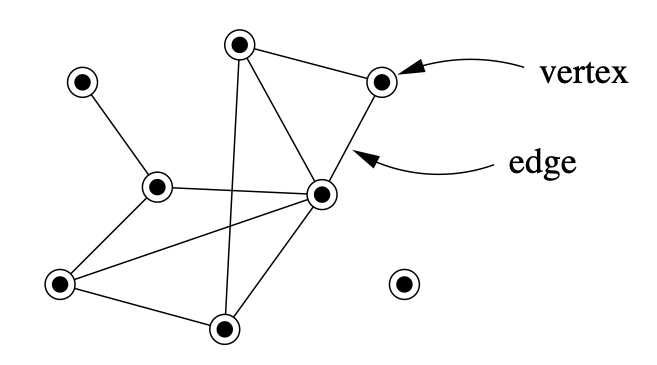
\includegraphics[width=0.5\linewidth,height=\textheight,keepaspectratio]{images/small-network.png}

There are a couple of things to be noted about this network, which we
will revisit later on. The links between the nodes do not have an
apparent directionality, making this an \textbf{undirected graph}. On
the other hand, when the direction between link is relevant, such as for
example in a predator-prey interaction, where it is convenient to
represent the fact that the flow of biomass runs from prey to predator,
the links might be represented as arrows. Networks represented in this
way are called \textbf{directed graphs}.

Secondly, one of the nodes is \emph{isolated}. Can you guess which one
it is?

You might have started noticing that depending on the types of links,
and their placement between nodes within the network, there are a few
categories under which we can classify networks according to their
features. Two categories are relevant for this course:

1.- Networks can be either \textbf{directed} or \textbf{undirected} as
we saw before.

2.- Depending on the constraints of connectivity between groups of
nodes, networks can be classified as either \textbf{unipartite} where
all nodes could in principle be connected to any other node, or
\textbf{bipartite}, where two different groups of nodes exist in which
\emph{links between nodes in different groups occur} but links between
nodes \emph{within the same group do not}.

We will encounter both \textbf{unipartite} and \textbf{bipartite}
networks along the way. Watch out!

Many systems both natural and man-made, can be thought of as networks.
From the network of airports around to world and the air routes
connecting them, to the World Wide Web and the links between web pages,
or social networks of friendships (both real and digital), all the way
down to microscopic entities such as gene and metabolic networks, these
systems can be represented and, perhaps more importantly, analysed as
networks.

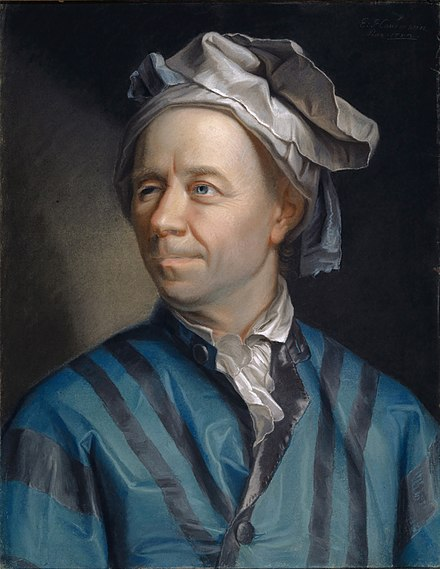
\includegraphics[width=2.91667in,height=\textheight,keepaspectratio]{images/Leonhard_Euler.jpeg}

The field of mathematics has been studying networks for decades. The
mathematics subfield of
\href{https://en.wikipedia.org/wiki/Graph_theory}{Graph Theory} has
developed extensive frameworks to analyse and manipulate mathematical
objects known as \texttt{graphs}. Graphs, as networks, are simply
collections of nodes and links between them. So, we can represent
networks as graphs and take advantage of the mathematical framework of
Graph Theory to study them.

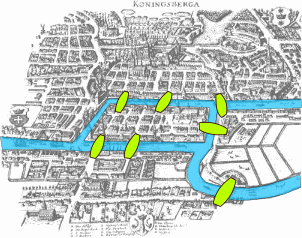
\includegraphics[width=3.95833in,height=\textheight,keepaspectratio]{images/konigsberg_bridges.png}

The mathematical study of graphs (or networks) arguably started in 1735
when the celebrated mathematician
\href{https://en.wikipedia.org/wiki/Leonhard_Euler}{Leonhard Euler},
yes!, the same one who introduced the \emph{e} as the base of the
natural logarithm, developed what is considered the first theorem of
graph theory to solve the problem known as the
\href{https://en.wikipedia.org/wiki/Seven_Bridges_of_K\%C3\%B6nigsberg}{Seven
bridges of Königsberg}.

Ever since then, the application of graph theory has percolated the
sciences. It started back in the 1930s when tools for the analysis of
networks were applied to the social sciences to develop a better
understanding of social relationships among humans.

In ecology, even though network representations of natural communities
can be traced back to the 1880's in the work by
\href{https://en.wikipedia.org/wiki/Lorenzo_Camerano}{Lorenzo Camerano},
the quantitative analysis of networks and their properties, as well as
their mathematical modelling, started much more recently, around the
1960's - 70's.

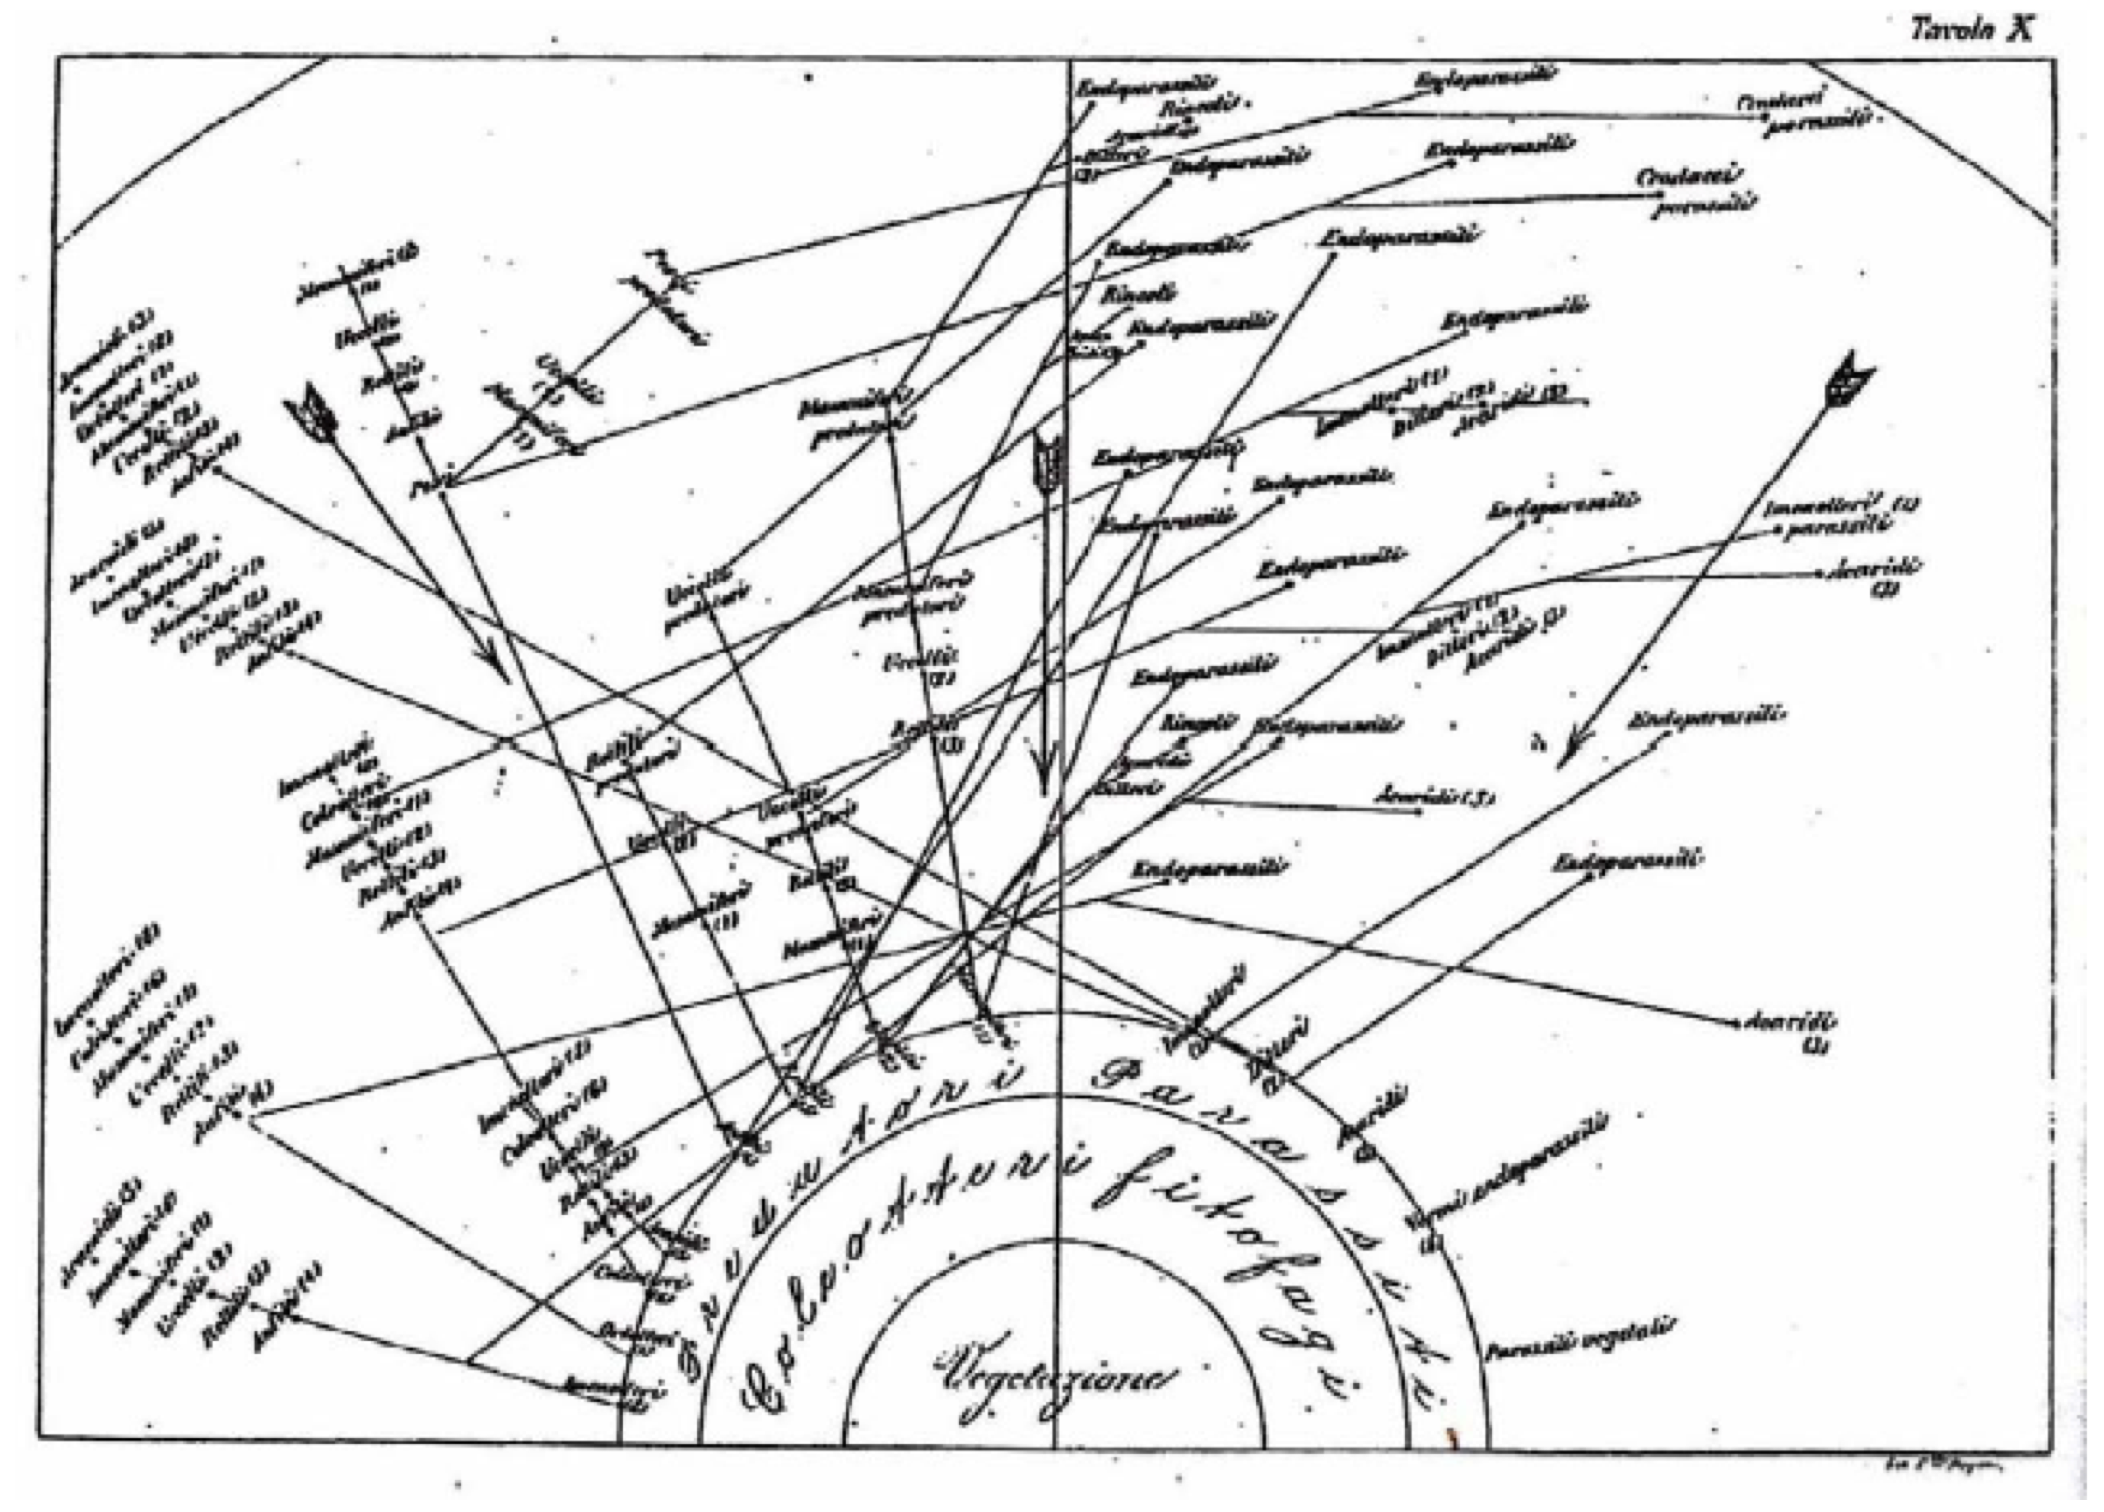
\includegraphics[width=3.95833in,height=\textheight,keepaspectratio]{images/camerano.png}

\textbf{Lorenzo Camerano's representation of a food web (1880)}

In the following sections we will learn how to analyse networks. Our
focus will be networks of ecological interactions between species
sharing the same ecological community. In very diverse systems these can
be up to 1,000's of species. As such, many of the quantities we will be
learning about are mostly relevant to quantify \textbf{biodiversity} and
can be seen as a natural extension to the classical analysis performed
in \textbf{community ecology}. Nonetheless, the underlying principles of
network construction and analysis can be applied to any networked
system, including those mentioned above.

\subsection{Network formats: edgelists and adjacency
matrices}\label{network-formats-edgelists-and-adjacency-matrices}

To be able to manipulate and analyse networks in an automated way, we
need to represent them in a way that is understandable by a computer.
Several computer readable formats exist to store the description and
information contained in a network. The most commonly used in ecology
(and other disciplines) are: (i) adjacency matrices, and (ii) edgelists.

\textbf{Adjancecy matrices}, one of the most common ways of representing
networks in mathematics, are matrices in which columns and rows
represent the nodes (species) in the network, and a link (interaction)
between them is represented as a 1, while the absence of a link is
represented as a 0.

In a foodweb, for example, as we saw previously, links are directed from
prey to predator. In the adjacency matrix, the rows represent prey
species and the columns represent predators. Thus, an interaction aij
runs from prey i to predator j.

\textbf{Adjacency matrices} are good for representing
\textbf{unipartite} networks because in principle there could be a
connection between any two nodes. In \textbf{bipartite} networks on the
other hand, as we saw before, we know in advance that some links cannot
occur (i.e.~those between nodes within the same groups). As such all
nodes do not have to be represented in each dimension of the matrix
(rows and columns) but only in one of them. This gives rise to a
slightly different format from an adjacency matrix, but where the
meaning of the elements in the matrix is still the same. These are
\textbf{incidence matrices}. In and \textbf{incidence matrix} one set of
nodes is represented by the rows and the other one by the columns. Links
thus connect nodes in the the rows with nodes in the columns. This makes
these matrices non-square.

An added virtue of the \textbf{incidence matrix} format is that it saves
us a lot of space in the computer (and in our notebooks if we were using
pen and paper!). Can you figure out why?

Can you think of a few examples of ecological networks that can be
represented as \textbf{bipartite} and thus as \textbf{incidence
matrices}?

That's right! Mutualistic networks (e.g.~plant-pollinator) are
bipartite. As such, they can be represented as incidence matrices, where
hosts are usually shown in rows and their mutualistic partners are shown
in columns.

\textbf{Edge lists}, on the other hand, are lists of pairs of
identifiers (usually integers) that denote links (or ecological
interactions) from the first item in pair to the second. For example, a
network specified by the following edge list:

1 2 2 3 1 3

is one with three nodes: V = \{1,2,3\}, and three links: one from basal
prey 1 to primary consumer 2, another one from prey (primary consumer) 2
to top predator 3, and finally, an interaction between the basal
resource and the top predator (E = \{(1,2), (2,3), (1,3)\}). This makes
the top predator an omnivorous species. A representation of this network
is shown below:

\pandocbounded{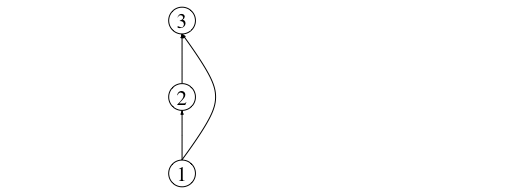
\includegraphics[keepaspectratio]{images/net1.png}}

This network can be represented as an adjacency matrix thus:

\pandocbounded{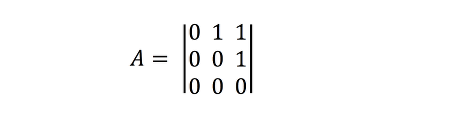
\includegraphics[keepaspectratio]{images/matrix.png}}

More sophisticated ways of representing and storing networks exist, such
as for example the \href{http://graphml.graphdrawing.org}{GraphML}
format, in which additional information about the network, the nodes,
and the links can be included in the description. During these lectures,
we will use a mixture of different formats to represent networks in text
files (e.g.~edge lists, adjacency matrices, etc).

Throughout the course we will use a few examples of real ecological
networks taken publicly available databases such as the well-known food
web from the Benguela upwelling marine system off the Western coast of
Africa:

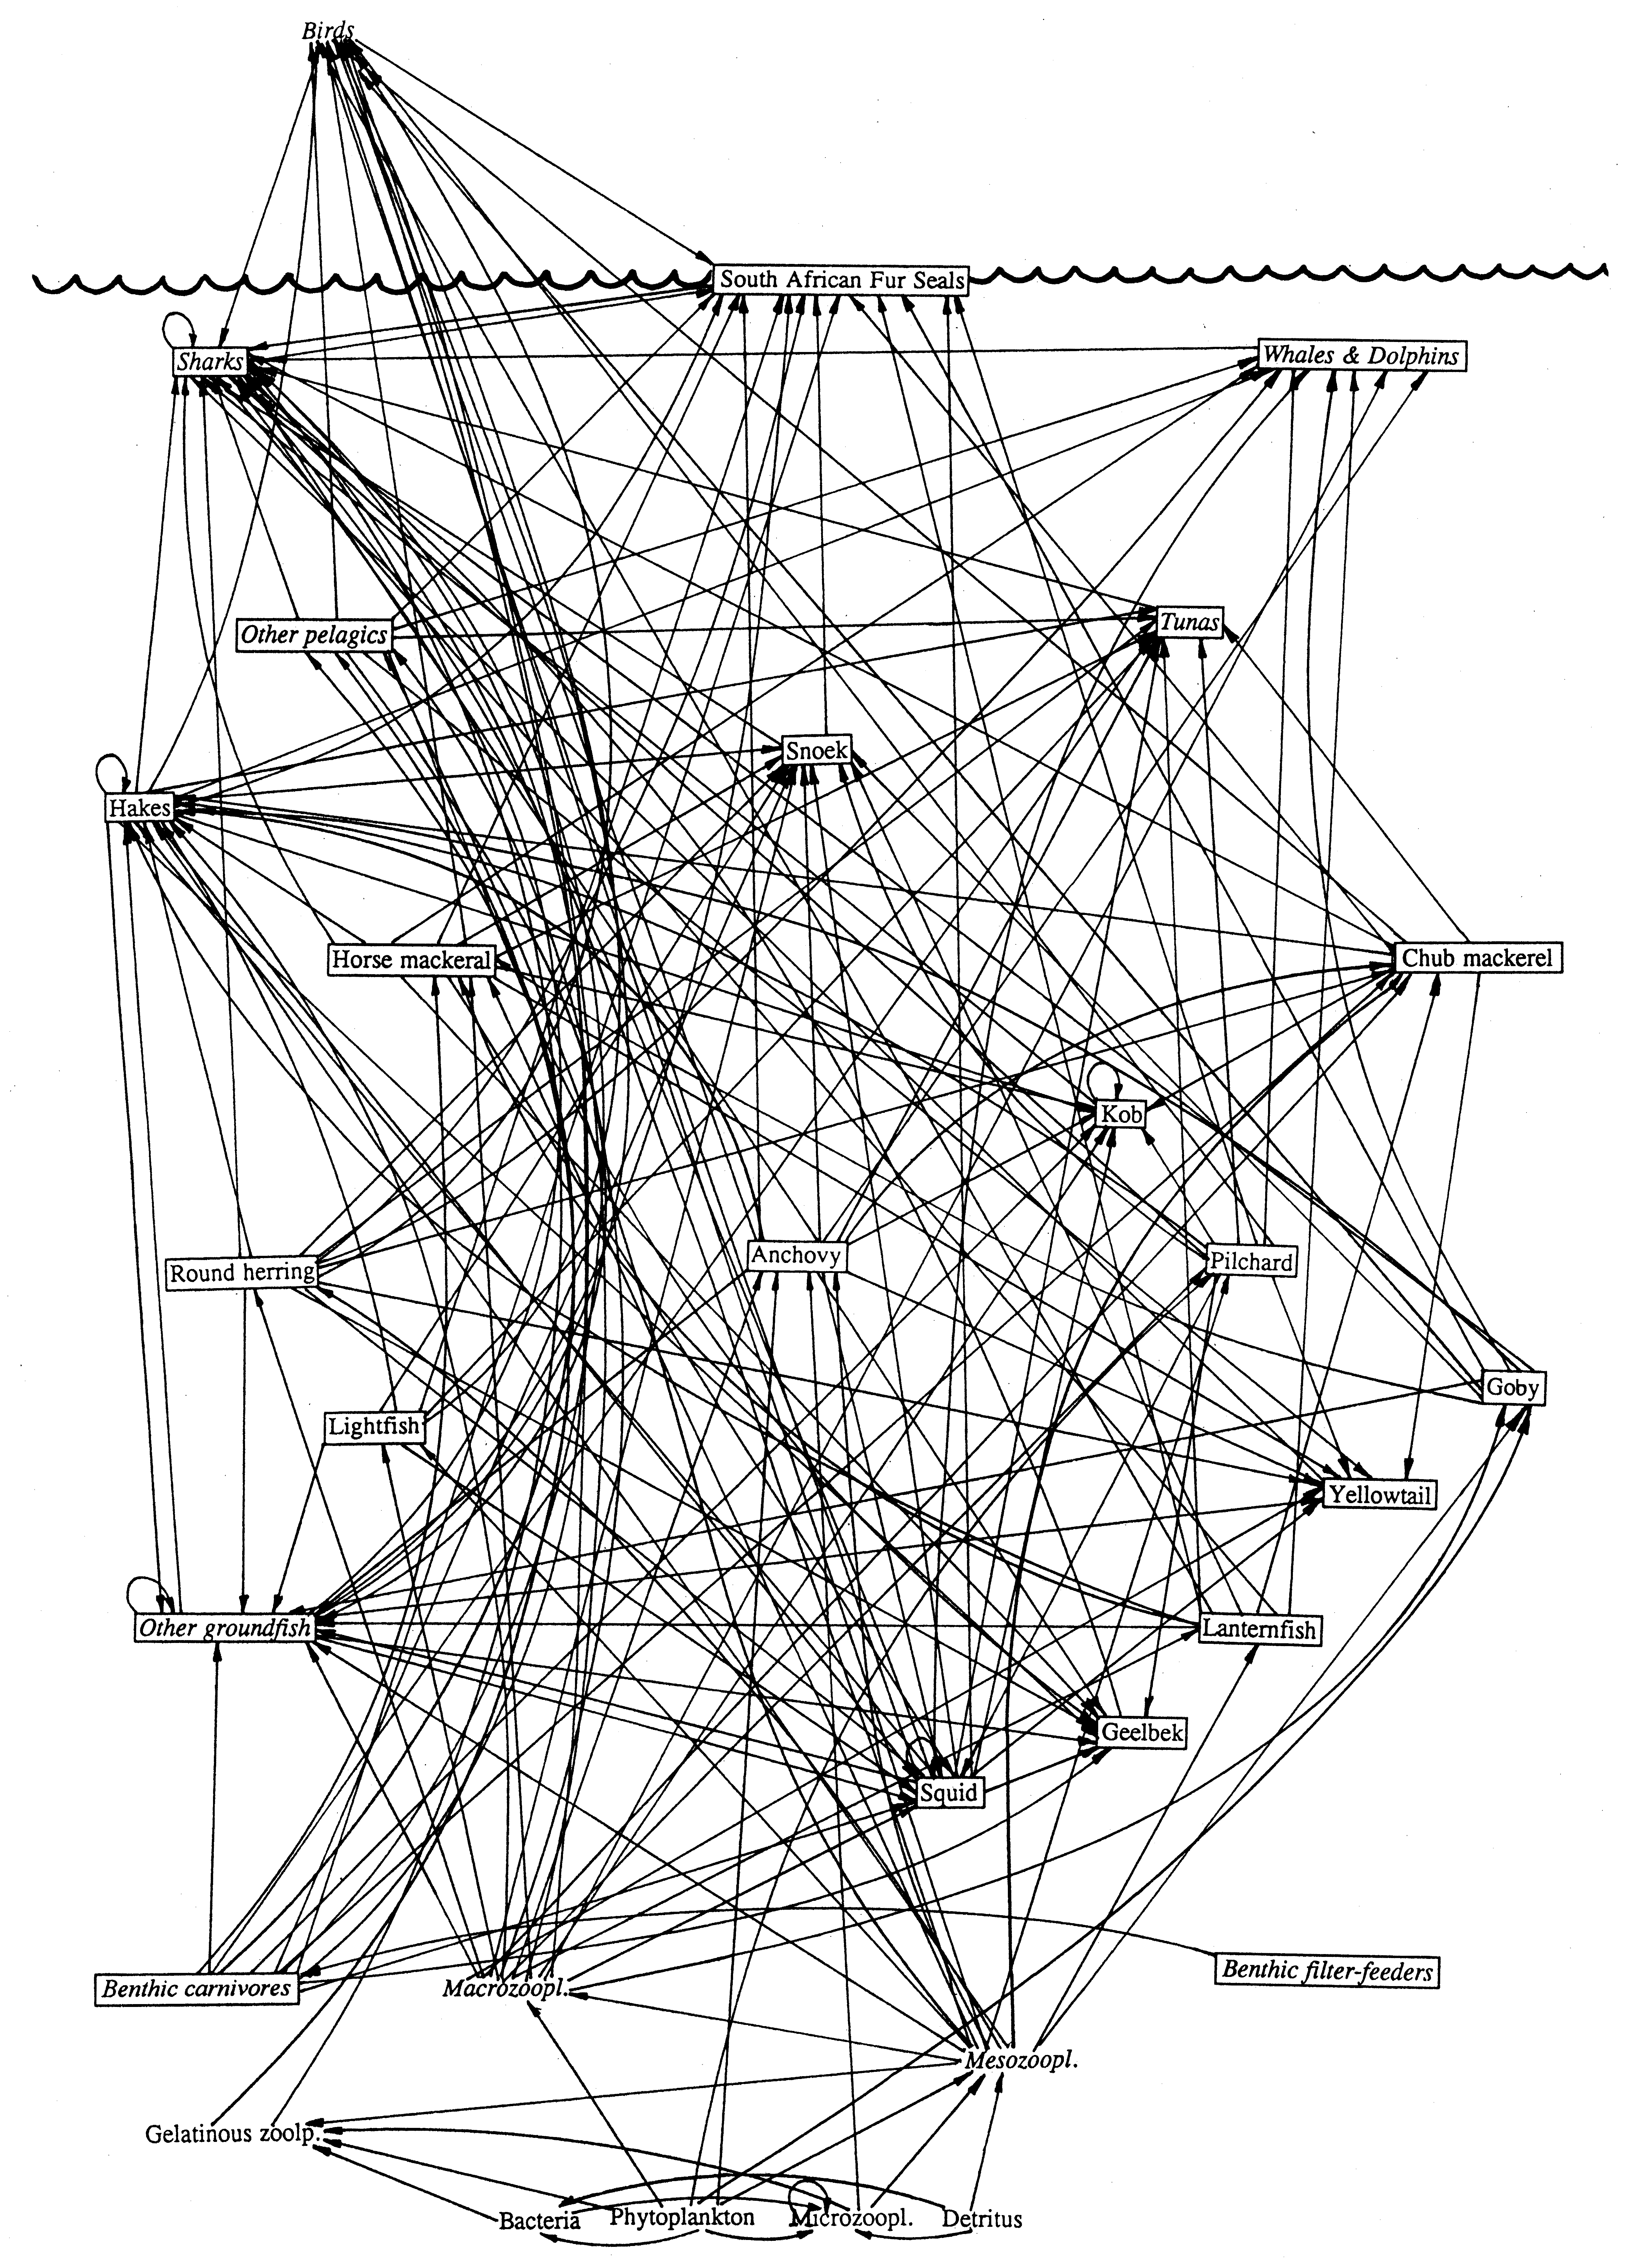
\includegraphics[width=\linewidth,height=5.20833in,keepaspectratio]{images/benguela.png}

Image taken from Yodzis, P (1998) \emph{Local trophodynamics and the
interaction of marine mammals and fisheries in the Benguela ecosystem}.
\textbf{Journal of Animal Ecology}. 67, 635-658.

This, and other ecological networks datasets, are available from the
\href{https://www.globalbioticinteractions.org/}{Global Biotic
Interactions Database GloBI}.

The code below will enable you to download the edgelist file and use it
to create an adjacency matrix representation of the network. Two
representations of the network then remain available: the Edgelist
representation (\texttt{benguela.EL}) and the Adjacency Matrix
representation (\texttt{benguela.AM}).

\begin{Shaded}
\begin{Highlighting}[]
\FunctionTok{library}\NormalTok{(RCurl)}
\NormalTok{x }\OtherTok{\textless{}{-}} \FunctionTok{getURL}\NormalTok{(}\StringTok{"https://raw.githubusercontent.com/mlurgi/networks\_for\_r/master/datasets/benguela.edgelist"}\NormalTok{)}
\NormalTok{benguela.EL }\OtherTok{\textless{}{-}} \FunctionTok{read.table}\NormalTok{(}\AttributeTok{text =}\NormalTok{ x) }
\NormalTok{benguela.EL }\OtherTok{\textless{}{-}} \FunctionTok{as.matrix}\NormalTok{(benguela.EL)}
\end{Highlighting}
\end{Shaded}

\begin{Shaded}
\begin{Highlighting}[]
\CommentTok{\# Create an adjacency matrix called benguela.AM, containing only zeros}
\NormalTok{benguela.AM }\OtherTok{\textless{}{-}} \FunctionTok{matrix}\NormalTok{(}\DecValTok{0}\NormalTok{, }\FunctionTok{max}\NormalTok{(benguela.EL), }\FunctionTok{max}\NormalTok{(benguela.EL))}

\CommentTok{\# Introduce ones to the matrix to represent interactions between species}
\NormalTok{benguela.AM[benguela.EL] }\OtherTok{\textless{}{-}} \DecValTok{1}
\end{Highlighting}
\end{Shaded}

\subsection{Species and interactions as vertices and
links}\label{species-and-interactions-as-vertices-and-links}

In abstract representations of ecological communities as networks, nodes
represent species and links amongst them denote ecological interactions
happening between the represented species.

\textbf{Adjacency matrices} are matrix representations of networks where
elements of the matrix denote the presence of a link (i.e.~interaction)
between the species represented by the row and the species represented
by the column. Thus, to represent a food web composed of S species as a
matrix we need a SxS matrix in order to be able to represent all
possible interaction between the S species. The number of species in the
network can be calculated thus as the number of rows or the number of
columns.

Using the Benguela food web adjacency matrix \texttt{benguela.AM}, you
can calculate the number of species.

In an adjacency matrix, all species are represented by columns and rows.
Counting the number of columns or rows in the adjacency matrix will let
you obtain the number of species in the food web. In R, you can use the
\texttt{dim} function to look at the matrix \textbf{dimensions}.

\begin{Shaded}
\begin{Highlighting}[]
\CommentTok{\# species richness}
\NormalTok{S }\OtherTok{\textless{}{-}} \FunctionTok{dim}\NormalTok{(benguela.AM)[}\DecValTok{1}\NormalTok{]}
\end{Highlighting}
\end{Shaded}

Similarly, since interactions are represented as ones in the matrix, if
you \texttt{sum} all the values in the matrix, you will get the number
of interactions.

\begin{Shaded}
\begin{Highlighting}[]
\CommentTok{\# number of links}
\NormalTok{L }\OtherTok{\textless{}{-}} \FunctionTok{sum}\NormalTok{(benguela.AM)}
\end{Highlighting}
\end{Shaded}

\subsection{Interactions in bipartite
networks}\label{interactions-in-bipartite-networks}

Food webs, like that for the Benguela ecosystem studied above, are
network representation of who eats whom relationships in an ecological
community. As such, there are no distinct subset of species among which
interactions are not possible. This is why adjacency matrices for
representing food webs contain the total number of species as rows and
also as columns. In theory, any interaction is possible.

Other types of ecological networks, however, like for example,
plant-animal mutualistic networks (like the figure below) or
host-parasite interaction networks, exhibit a bipartite structure. In
this type of networks, species can be classified into two distinct
groups where interactions do not occur (or are forbidden) among members
of the same group. For example, in a plant-animal mutualistic network,
plants do not interact with plants and animal mutualists do not interact
among them. This feature allows for a more concise matrix representation
of bipartite networks.

\pandocbounded{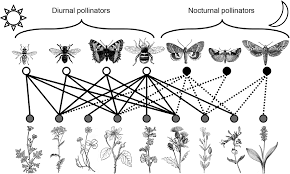
\includegraphics[keepaspectratio]{images/plant-pollinator.png}}

\textbf{Example of a plant-animal pollinator bipartite network.} Image
taken from MacGregor, CJ et al.~(2015) \emph{Pollination by nocturnal
Lepidoptera, and the effects of light pollution, a review}.
\textbf{Ecological Entomology}. 40, 187-198.

As we saw above, the equivalent representation of an adjacency matrix
for a bipartite network is called an incidence matrix. In incidence
matrices one set of species are represented as rows (e.g.~hosts/plants),
and the other set of species as columns (e.g.~visitors/mutualists).
Thus, the way of counting species in an incidence matrix representing a
mutualistic (bipartite) network is different from that used to count
species in adjacency matrices representing food webs.

For a bipartite ecological network represented by an incidence matrix
with size HxV, where H is the number of rows and V is the number of
columns, the number of species in the network is equal to H + V.

As an example, we load a matrix representing a bipartite network of
interactions between anemones and several species of fish living within
them in South-East Asia. This network was taken from Ollerton, J. et
al.~(2007) \emph{Finding NEMO: nestedness engendered by mutualistic
organization in anemonefish and their hosts}. \textbf{Proceedings of the
Royal Society B}. 274, 591-598.

Try and calculate the total number of anemone \emph{and} fish species in
the network. Remember that in a bipartite network, one set of species
(in this case, anemones) are represented as columns, while the other set
(in this case, fishes) are represented as rows.

\begin{Shaded}
\begin{Highlighting}[]
\FunctionTok{library}\NormalTok{(RCurl)}
\NormalTok{y }\OtherTok{\textless{}{-}} \FunctionTok{getURL}\NormalTok{(}\StringTok{"https://raw.githubusercontent.com/mlurgi/networks\_for\_r/master/datasets/anemonefish.txt"}\NormalTok{)}
\NormalTok{anemonef }\OtherTok{\textless{}{-}} \FunctionTok{read.table}\NormalTok{(}\AttributeTok{text =}\NormalTok{ y)}
\FunctionTok{names}\NormalTok{(anemonef) }\OtherTok{\textless{}{-}} \FunctionTok{paste}\NormalTok{(}\StringTok{"A"}\NormalTok{, }\DecValTok{1}\SpecialCharTok{:}\DecValTok{10}\NormalTok{, }\AttributeTok{sep =} \StringTok{""}\NormalTok{)}
\FunctionTok{row.names}\NormalTok{(anemonef) }\OtherTok{\textless{}{-}} \FunctionTok{paste}\NormalTok{(}\StringTok{"F"}\NormalTok{, }\DecValTok{1}\SpecialCharTok{:}\DecValTok{26}\NormalTok{, }\AttributeTok{sep =} \StringTok{""}\NormalTok{)       }
\NormalTok{anemonef }\OtherTok{\textless{}{-}} \FunctionTok{as.matrix}\NormalTok{(anemonef)}

\DocumentationTok{\#\#\# The number of fish species in the network is the number of rows}
\NormalTok{n\_fish }\OtherTok{\textless{}{-}} \FunctionTok{dim}\NormalTok{(anemonef)[}\DecValTok{1}\NormalTok{]}
\DocumentationTok{\#\#\# The number of anemone species is the number of columns}
\NormalTok{n\_anemone }\OtherTok{\textless{}{-}} \FunctionTok{dim}\NormalTok{(anemonef)[}\DecValTok{2}\NormalTok{]}

\DocumentationTok{\#\#\# So, the total number of species is the sum of these two quantities}
\NormalTok{S }\OtherTok{\textless{}{-}}\NormalTok{ n\_fish }\SpecialCharTok{+}\NormalTok{ n\_anemone}

\DocumentationTok{\#\#\# Whereas the total number of interactions is still the sum of the matrix}
\NormalTok{L }\OtherTok{\textless{}{-}} \FunctionTok{sum}\NormalTok{(anemonef)}
\end{Highlighting}
\end{Shaded}

\subsection{Networks as graphs}\label{networks-as-graphs}

As we have seen, edge lists and adjacency matrices are convenient ways
in which interaction networks can be represented. However, more flexible
formats for representing networks are needed when we want to perform
more complex actions on networks, or even just for visualisation
purposes.

Several computer programming libraries have been especially developed to
construct and manipulate graphs. These libraries make it easy and widely
accessible to work with and study networks. Amongst the most popular the
\href{https://networkx.github.io/}{NetworkX} complex networks library
for \href{https://www.python.org/}{Python} and the
\href{https://igraph.org/}{igraph} package for network analysis, which
can be used on several platforms, including
\href{https://www.r-project.org/}{R}. For the rest of this course we
will be using \texttt{igraph} to create and manipulate ecological
networks.

To install and load igraph on your R workspace run the following
commands:

\begin{Shaded}
\begin{Highlighting}[]
\DocumentationTok{\#\# Install igraph}
\FunctionTok{install.packages}\NormalTok{(}\StringTok{"igraph"}\NormalTok{)}

\DocumentationTok{\#\# Load igraph into workspace}
\FunctionTok{library}\NormalTok{(igraph)}
\end{Highlighting}
\end{Shaded}

To start getting familiar with igraph we will start by creating some
simple networks.

\subsubsection{Weaving networks from
scratch}\label{weaving-networks-from-scratch}

The following instructions will walk you through a simple example in
which you will create a small network:

1.- First create a vector called \texttt{species} with the numbers from
1 to 10

2.- Then create a network by adding the \texttt{species} as
\texttt{vertices} to an empty graph

3.- Create an interaction between species 5 and 7

4.- Create 10 other interactions between any species you want

\begin{Shaded}
\begin{Highlighting}[]
\FunctionTok{require}\NormalTok{(igraph)}
\CommentTok{\# Ten species}
\NormalTok{species }\OtherTok{\textless{}{-}} \DecValTok{1}\SpecialCharTok{:}\DecValTok{10}
\NormalTok{network }\OtherTok{\textless{}{-}} \FunctionTok{graph.empty}\NormalTok{() }\SpecialCharTok{+} \FunctionTok{vertices}\NormalTok{(species)}

\CommentTok{\# Link between species 5 and 7}
\NormalTok{network[}\DecValTok{5}\NormalTok{,}\DecValTok{7}\NormalTok{] }\OtherTok{\textless{}{-}} \DecValTok{1}
\end{Highlighting}
\end{Shaded}

\subsubsection{Converting matrix to igraph
object}\label{converting-matrix-to-igraph-object}

If we have an adjacency matrix and we want an igraph object representing
the same network, without the need to create the network from scratch,
igraph offers the functionality of creating graphs from adjacency
matrices. Just use the function
\texttt{graph\_from\_adjacency\_matrix(A)}, where A is your adjacency
matrix.

Check out the documentation for
\href{http://igraph.org/r/doc/graph_from_adjacency_matrix.html}{graph.adjacency},
including additional parameters that you can use to create your network.
Similarly, to create a graph from an edgelist, you can use the
\texttt{graph\_from\_edgelist}function from igraph.

We can convert the network for the Benguela ecosystem, into and igraph
object using the following code.

\begin{Shaded}
\begin{Highlighting}[]
\FunctionTok{library}\NormalTok{(RCurl)}
\NormalTok{x }\OtherTok{\textless{}{-}} \FunctionTok{getURL}\NormalTok{(}\StringTok{"https://raw.githubusercontent.com/mlurgi/networks\_for\_r/master/datasets/benguela.edgelist"}\NormalTok{)}
\NormalTok{benguela.EL }\OtherTok{\textless{}{-}} \FunctionTok{read.table}\NormalTok{(}\AttributeTok{text =}\NormalTok{ x) }
\NormalTok{benguela.EL }\OtherTok{\textless{}{-}} \FunctionTok{as.matrix}\NormalTok{(benguela.EL)}

\CommentTok{\# Create an adjacency matrix called benguela.AM, containing only zeros}
\NormalTok{benguela.AM }\OtherTok{\textless{}{-}} \FunctionTok{matrix}\NormalTok{(}\DecValTok{0}\NormalTok{, }\FunctionTok{max}\NormalTok{(benguela.EL), }\FunctionTok{max}\NormalTok{(benguela.EL))}

\CommentTok{\# Introduce ones to the matrix to represent interactions between species}
\NormalTok{benguela.AM[benguela.EL] }\OtherTok{\textless{}{-}} \DecValTok{1}

\CommentTok{\# Convert Benguela adjacency matrix to an igraph network}
\NormalTok{benguela.network }\OtherTok{\textless{}{-}} \FunctionTok{graph\_from\_adjacency\_matrix}\NormalTok{(benguela.AM)}
\end{Highlighting}
\end{Shaded}

\subsubsection{Drawing networks}\label{drawing-networks}

The network representations we have explored so far are great for
manipulating them and calculating properties over them. However, to gain
an intuitive idea of what the networks we are analysing look like, or if
we want to show them in publications or websites, it is sometimes
desirable to draw them as graphs: with dots representing nodes/species
and lines connecting them representing links/interactions. In pretty
much the same way we saw in the introductory video.

Of course, drawing a network on a whiteboard using coloured pens is
easy. Doing that on a computer or writing code in R to do it, might be
more of a challenge. Fortunately, libraries such as igraph offer these
functionalities. The
\href{http://igraph.org/r/doc/plot.igraph.html}{plot} function from the
igraph library takes as an input an igraph object and produces a
graphical representation of the network.

Let's try it!

\begin{Shaded}
\begin{Highlighting}[]
\CommentTok{\# Plotting your network}
\FunctionTok{plot}\NormalTok{(network)}
\end{Highlighting}
\end{Shaded}

If the instructions above worked well you will be able to see something
like this:

\pandocbounded{
\includegraphics[keepaspectratio]{lesson-images/first-network.png}}

What about the Benguela ecosystem network\ldots{}

\begin{Shaded}
\begin{Highlighting}[]
\CommentTok{\# Plot the Benguela food web}
\FunctionTok{plot}\NormalTok{(benguela.network, }\AttributeTok{edge.arrow.size =} \FloatTok{0.2}\NormalTok{)}
\end{Highlighting}
\end{Shaded}

\pandocbounded{\includegraphics[keepaspectratio]{networks-session_files/figure-latex/unnamed-chunk-10-1.pdf}}

This representation of the Benguela web looks a bit messy. Don't worry!
We will explore ways of making networks more beautiful later on.

\subsection{Network Properties}\label{network-properties}

Now that we have an igraph representation of our network(s), we can
calculate several of its properties.

\subsubsection{Graph connectivity / Food web
connectance}\label{graph-connectivity-food-web-connectance}

If we think of the network we just constructed as a food web, we can
calculate the number of species and links (what we did previously on
adjacency matrices) thus:

\begin{Shaded}
\begin{Highlighting}[]
\CommentTok{\# number of species}
\NormalTok{S }\OtherTok{\textless{}{-}} \FunctionTok{vcount}\NormalTok{(network)}

\CommentTok{\# number of interactions}
\NormalTok{L }\OtherTok{\textless{}{-}} \FunctionTok{ecount}\NormalTok{(network)}
\end{Highlighting}
\end{Shaded}

The functions \texttt{vcount} and \texttt{ecount} from the igraph
library let you count the number of nodes and links on a graph,
respectively.

Having counted the number of species and links in our newly built food
web, we can start calculating more interesting prorperties such as
connectivity. In food webs connectivity can be quantified as the average
number of interactions per species (L/S, i.e.~the mean number of
interactions species in the network have), and \texttt{Connectance}
(L/S\textsuperscript{2}, i.e.~the fraction of links present in the
network out of all possible links).

\begin{Shaded}
\begin{Highlighting}[]
\CommentTok{\# average number of interactions species}
\NormalTok{L.S }\OtherTok{\textless{}{-}}\NormalTok{ L}\SpecialCharTok{/}\NormalTok{S}

\CommentTok{\# food web connectance}
\NormalTok{C }\OtherTok{\textless{}{-}}\NormalTok{ L}\SpecialCharTok{/}\NormalTok{S}\SpecialCharTok{\^{}}\DecValTok{2}
\end{Highlighting}
\end{Shaded}

In the case of the adjacency matrix (A) representation of a food web, we
know that it contains all the links in our network represented by 1's.
Hence, the number of links in our network is simply sum(A). Similarly we
have also learnt that the number of species (at least for a food web)
equals the number of rows (or columns) in the matrix: nrow(A).

Hence, the connectance of our food web represented by matrix A is
calculated as: sum(A)/(nrow(A)\textsuperscript{2}). Try this on your
network above and you should obtain the same quantity we now have in
\texttt{C}. \textbf{HINT:} To obtain the adjacency matrix representation
of an igraph object you can use the \texttt{as\_adjacency\_matrix}
function.

For the Benguela network we can calculate connectivity properties:

\begin{Shaded}
\begin{Highlighting}[]
\CommentTok{\# Calculate connectance}
\NormalTok{connectance }\OtherTok{\textless{}{-}} \FunctionTok{ecount}\NormalTok{(benguela.network) }\SpecialCharTok{/} \FunctionTok{vcount}\NormalTok{(benguela.network)}\SpecialCharTok{\^{}}\DecValTok{2} 

\CommentTok{\# Print connectance}
\FunctionTok{print}\NormalTok{(}\FunctionTok{paste0}\NormalTok{(}\StringTok{\textquotesingle{}Connectance of Benguela network = \textquotesingle{}}\NormalTok{, }\FunctionTok{round}\NormalTok{(connectance,}\DecValTok{2}\NormalTok{)))}
\end{Highlighting}
\end{Shaded}

\begin{verbatim}
## [1] "Connectance of Benguela network = 0.25"
\end{verbatim}

\begin{Shaded}
\begin{Highlighting}[]
\CommentTok{\# Calculate number of links per species}
\NormalTok{links.per.species }\OtherTok{\textless{}{-}} \FunctionTok{ecount}\NormalTok{(benguela.network) }\SpecialCharTok{/} \FunctionTok{vcount}\NormalTok{(benguela.network)}
\end{Highlighting}
\end{Shaded}

\subsubsection{Connectance in bipartite
networks}\label{connectance-in-bipartite-networks}

We have learnt how to calculate the connectance of ecological networks
in general: it is simply the fraction of realised links out of the
possible ones. Additionally, we have explored methods to quantify
connectance in food webs based on the information extracted either from
the adjacency matrix or the igraph representation of our networks.

We have also learnt that the way in which bipartite networks are
represented in incidence matrices is fundamentally different from the
way in which we represent food webs in adjacency matrices. Keeping that
in mind, we need to find out ways of finding out what would be: 1.- the
correct way of finding out the number of species in a bipartite network
from our matrix representation; and 2.- the total possible number of
links in a bipartite network (remember that links between species in the
same group are `forbidden').

Using the fish-anemone interaction network that we used previously, we
can calculate the total number of possible links as the product of the
number of species on one side (i.e.~fish) times the number of species on
the other side (i.e.~anemone). This will give us the total number of
links if every fish species would be found to interact with each anemone
species. Connectance of this network is then simply the total number of
links divided by this quantity.

\begin{Shaded}
\begin{Highlighting}[]
\FunctionTok{library}\NormalTok{(RCurl)}
\NormalTok{y }\OtherTok{\textless{}{-}} \FunctionTok{getURL}\NormalTok{(}\StringTok{"https://raw.githubusercontent.com/seblun/networks\_datacamp/master/datasets/anemonefish.txt"}\NormalTok{)}
\NormalTok{anemonef }\OtherTok{\textless{}{-}} \FunctionTok{read.table}\NormalTok{(}\AttributeTok{text =}\NormalTok{ y)}
\FunctionTok{names}\NormalTok{(anemonef) }\OtherTok{\textless{}{-}} \FunctionTok{paste}\NormalTok{(}\StringTok{"A"}\NormalTok{, }\DecValTok{1}\SpecialCharTok{:}\DecValTok{10}\NormalTok{, }\AttributeTok{sep =} \StringTok{""}\NormalTok{)}
\FunctionTok{row.names}\NormalTok{(anemonef) }\OtherTok{\textless{}{-}} \FunctionTok{paste}\NormalTok{(}\StringTok{"F"}\NormalTok{, }\DecValTok{1}\SpecialCharTok{:}\DecValTok{26}\NormalTok{, }\AttributeTok{sep =} \StringTok{""}\NormalTok{)       }
\NormalTok{anemonef }\OtherTok{\textless{}{-}} \FunctionTok{as.matrix}\NormalTok{(anemonef)}

\CommentTok{\# Calculate conectance of anemonef}
\NormalTok{bipartite.connectance }\OtherTok{\textless{}{-}} \FunctionTok{sum}\NormalTok{(anemonef) }\SpecialCharTok{/}\NormalTok{ (}\FunctionTok{dim}\NormalTok{(anemonef)[}\DecValTok{1}\NormalTok{] }\SpecialCharTok{*} \FunctionTok{dim}\NormalTok{(anemonef)[}\DecValTok{2}\NormalTok{])}
      
\FunctionTok{print}\NormalTok{(}\FunctionTok{paste0}\NormalTok{(}\StringTok{\textquotesingle{}Connectance of the bipartite anemonefish network = \textquotesingle{}}\NormalTok{, }\FunctionTok{round}\NormalTok{(bipartite.connectance,}\DecValTok{2}\NormalTok{)))}
\end{Highlighting}
\end{Shaded}

\begin{verbatim}
## [1] "Connectance of the bipartite anemonefish network = 0.31"
\end{verbatim}

Igraph lets us manipulate bipartite networks in a similar way to
unipartite ones. We can load the incidence matrix above using the
following instruction:

\begin{Shaded}
\begin{Highlighting}[]
\NormalTok{anemonef.network }\OtherTok{\textless{}{-}} \FunctionTok{graph\_from\_biadjacency\_matrix}\NormalTok{(anemonef, }\AttributeTok{directed =} \ConstantTok{TRUE}\NormalTok{, }\AttributeTok{mode =} \StringTok{\textquotesingle{}in\textquotesingle{}}\NormalTok{)}
\end{Highlighting}
\end{Shaded}

And calculate its connectance thus:

\begin{Shaded}
\begin{Highlighting}[]
\CommentTok{\# Calculate conectance of anemoref}
\NormalTok{bipartite.connectance }\OtherTok{\textless{}{-}} \FunctionTok{ecount}\NormalTok{(anemonef.network) }\SpecialCharTok{/}\NormalTok{ (}\FunctionTok{sum}\NormalTok{(}\FunctionTok{V}\NormalTok{(anemonef.network)}\SpecialCharTok{$}\NormalTok{type) }\SpecialCharTok{*}\NormalTok{ (}\FunctionTok{vcount}\NormalTok{(anemonef.network) }\SpecialCharTok{{-}} \FunctionTok{sum}\NormalTok{(}\FunctionTok{V}\NormalTok{(anemonef.network)}\SpecialCharTok{$}\NormalTok{type)) )}
\end{Highlighting}
\end{Shaded}

As a fun exercise you can try and calculate the average number of links
per species in this network!

Aside from the connectivity measures that we learnt in the previous
section, more interesting properties can be calculated on ecological
networks. In this chapter, we introduce some of these properties and how
to calculate them.

\subsubsection{Horizontal Diversity : Generality and
Vulnerability}\label{horizontal-diversity-generality-and-vulnerability}

Ecological networks are all about species and their interactions. In
food webs, these interactions represent consumer-resource relationships,
so the set of relationships that a consumer has with its prey is
considered the `breadth' of its diet. This diet breadth is a measure of
the generality of the consumer species and a mean generality index can
be calculated across the network to have an idea of how generalist are
species in the network on average. We can calculate generality on the
matrix representation of our food webs using the following function:

\begin{Shaded}
\begin{Highlighting}[]
\DocumentationTok{\#\# Mean generality of species in the network}
\NormalTok{Generality }\OtherTok{\textless{}{-}} \ControlFlowTok{function}\NormalTok{(M)\{}
  \FunctionTok{return}\NormalTok{(}\FunctionTok{sum}\NormalTok{(}\FunctionTok{colSums}\NormalTok{(M))}\SpecialCharTok{/}\FunctionTok{sum}\NormalTok{((}\FunctionTok{colSums}\NormalTok{(M)}\SpecialCharTok{!=}\DecValTok{0}\NormalTok{)));}
\NormalTok{\}}
\end{Highlighting}
\end{Shaded}

Similarly, we can obtain a measure of the average number of consumers
that resources on our networks have (i.e.~vulnerability) using the
following function on our adjacency matrix:

\begin{Shaded}
\begin{Highlighting}[]
\DocumentationTok{\#\# Mean vulnerability of the species in the network}
\NormalTok{Vulnerability }\OtherTok{\textless{}{-}} \ControlFlowTok{function}\NormalTok{(M)\{}
  \FunctionTok{return}\NormalTok{(}\FunctionTok{sum}\NormalTok{(}\FunctionTok{rowSums}\NormalTok{(M))}\SpecialCharTok{/}\FunctionTok{sum}\NormalTok{((}\FunctionTok{rowSums}\NormalTok{(M)}\SpecialCharTok{!=}\DecValTok{0}\NormalTok{)));}
\NormalTok{\}}
\end{Highlighting}
\end{Shaded}

To be able to compare these quantities across different networks, they
are usually normalised by the average number of links per species
(\texttt{L/S}).

If we are interested in these quantities at the species level, we simply
count their prey or predator numbers or their \texttt{degree} in the
network:

\begin{Shaded}
\begin{Highlighting}[]
\DocumentationTok{\#\# In{-}degree or number of prey of all species in the network}
\NormalTok{InDegree }\OtherTok{\textless{}{-}} \ControlFlowTok{function}\NormalTok{(M)\{}
  \FunctionTok{return}\NormalTok{(}\FunctionTok{colSums}\NormalTok{(M));}
\NormalTok{\}}

\DocumentationTok{\#\# Out{-}degree or number of predators of all species in the network}
\NormalTok{OutDegree }\OtherTok{\textless{}{-}} \ControlFlowTok{function}\NormalTok{(M)\{}
  \FunctionTok{return}\NormalTok{(}\FunctionTok{rowSums}\NormalTok{(M));}
\NormalTok{\}}
\end{Highlighting}
\end{Shaded}

Even though these measures are useful to have an idea of the average
diet breadth and number of consumers across species in our networks, in
many occasions it is desirable to look at the deviation of these
properties, since we can have within the same network generalist species
such as this guy on the left\ldots{} \ldots{} alongside very specialist
species, such as this guy on the right\ldots{}

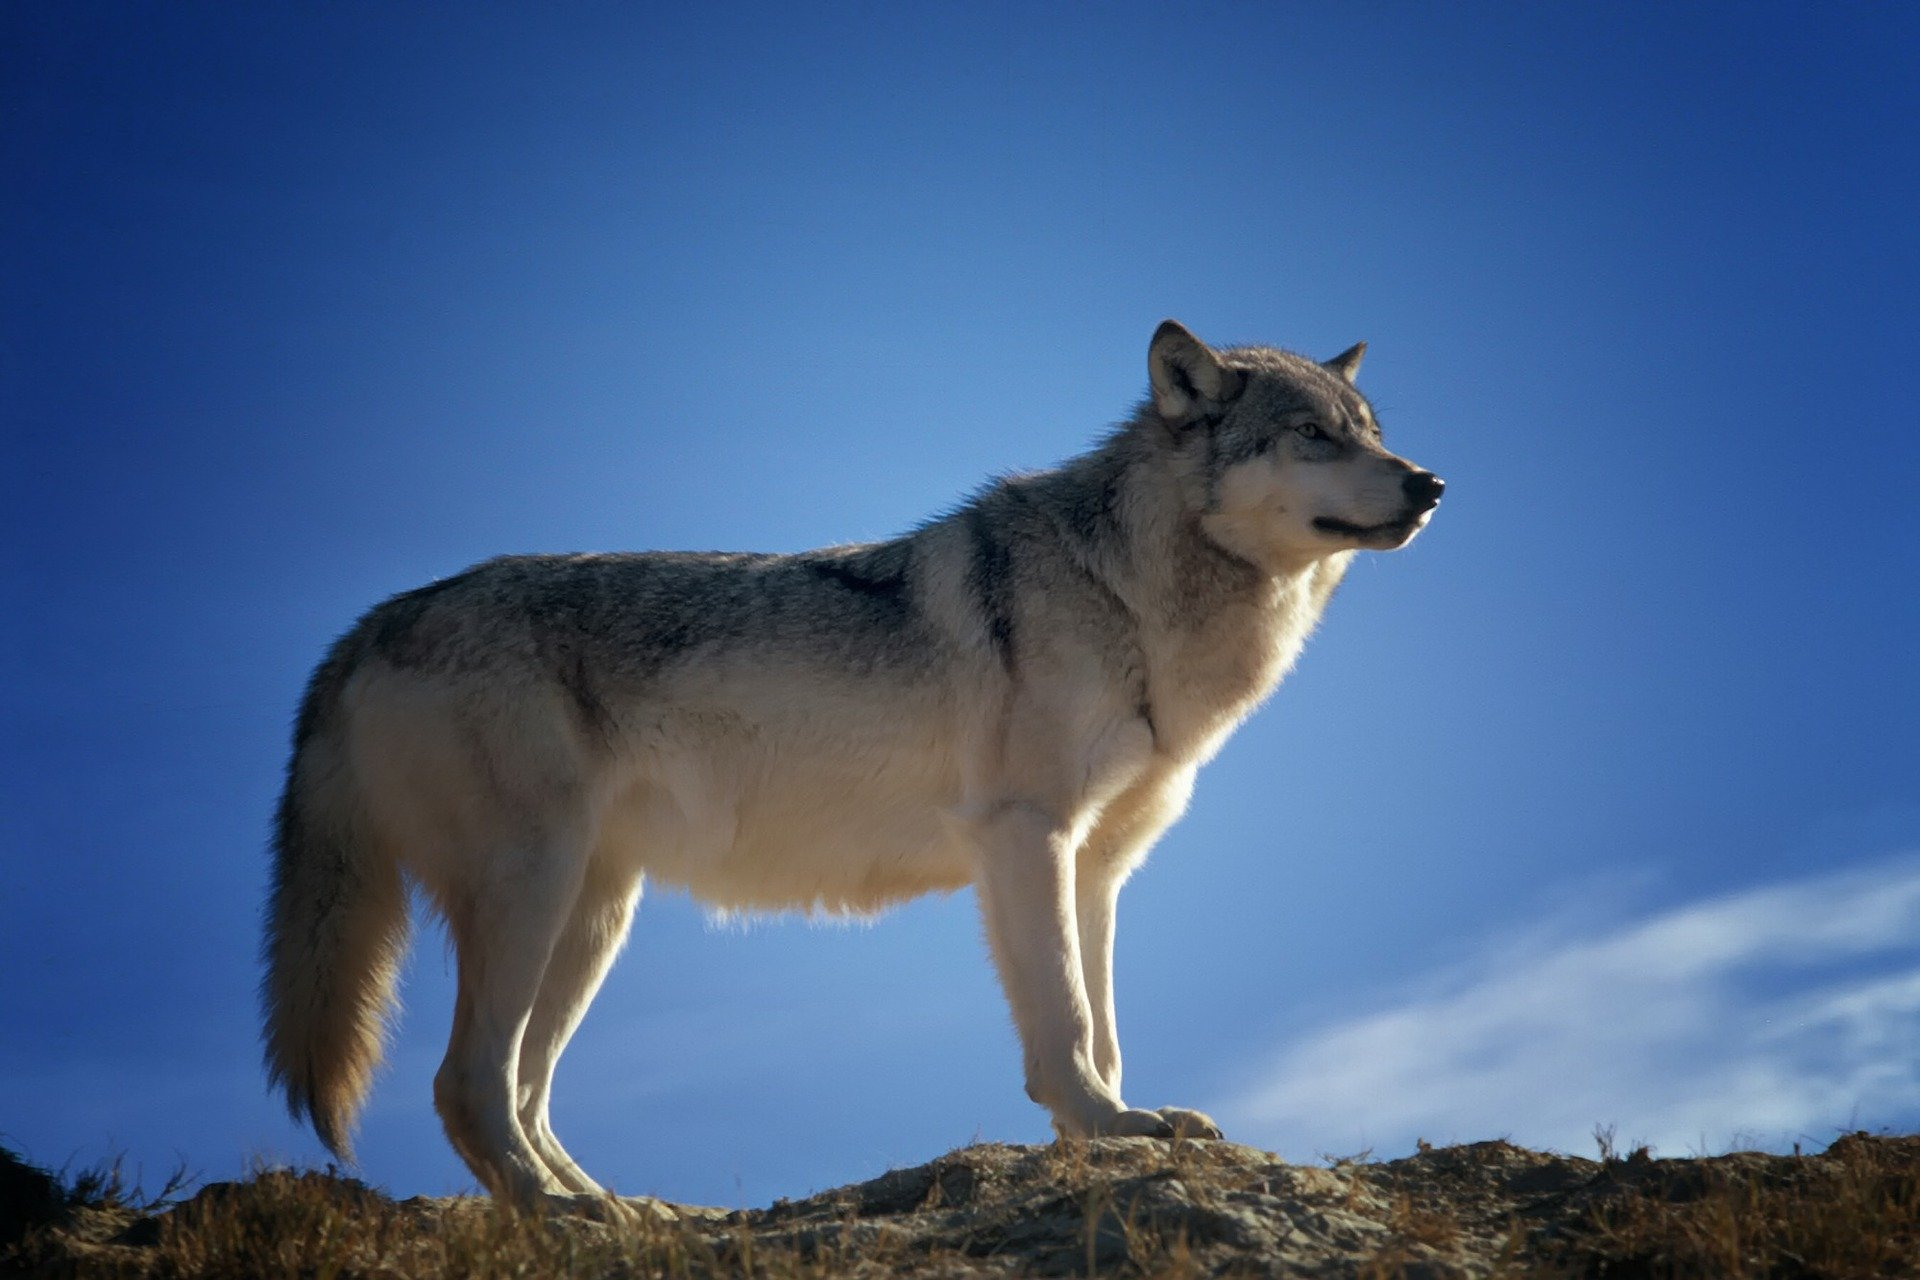
\includegraphics[width=3.38542in,height=\textheight,keepaspectratio]{images/wolf.jpg}
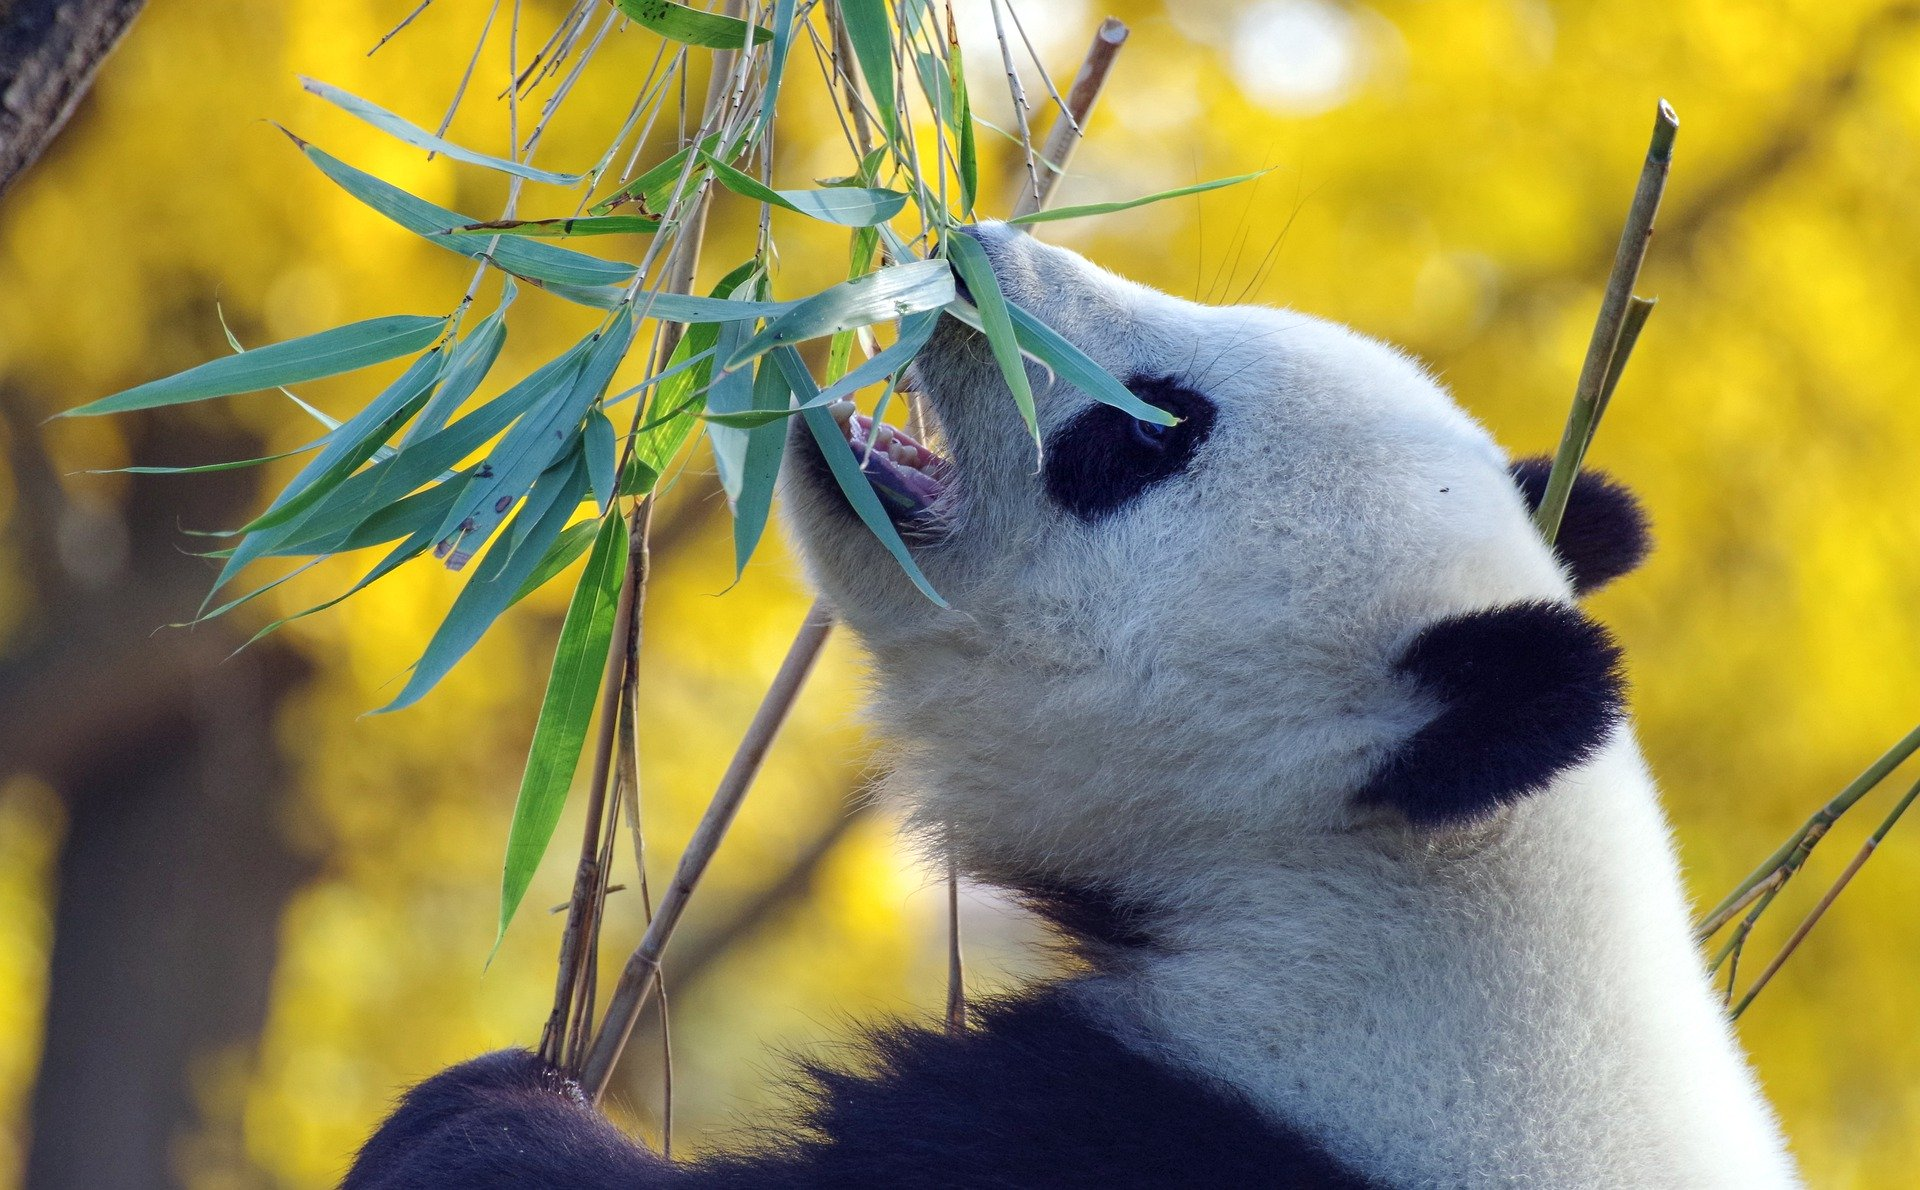
\includegraphics[width=3.64583in,height=\textheight,keepaspectratio]{images/panda.jpg}

To assess variability in diet breadth and the degree of vulnerability of
species in a food web, metrics such as the standard deviation of
normalised generality and vulnerability are useful. These properties can
be calculated using the following formulae:

\[G_{i}=\frac{1}{L/S}\sum_{j=1}^{S}a_{ji}\]
\[V_{i}=\frac{1}{L/S}\sum_{j=1}^{S}a_{ij}\]

where aij are the i,j values of the adjacency matrix \texttt{A}
representing the food web.

Using R code they can be calculated thus:

\begin{Shaded}
\begin{Highlighting}[]
\DocumentationTok{\#\# Standard deviation of generality:}
\NormalTok{SDGenerality }\OtherTok{\textless{}{-}} \ControlFlowTok{function}\NormalTok{(M)\{}
  \FunctionTok{return}\NormalTok{(}\FunctionTok{sd}\NormalTok{(}\FunctionTok{colSums}\NormalTok{(M) }\SpecialCharTok{/}\NormalTok{ (}\FunctionTok{sum}\NormalTok{(M)}\SpecialCharTok{/}\FunctionTok{dim}\NormalTok{(M)[}\DecValTok{1}\NormalTok{]) ));}
\NormalTok{\}}

\DocumentationTok{\#\# Standard deviation of vulnerability:}
\NormalTok{SDVulnerability }\OtherTok{\textless{}{-}} \ControlFlowTok{function}\NormalTok{(M)\{}
  \FunctionTok{return}\NormalTok{(}\FunctionTok{sd}\NormalTok{(}\FunctionTok{rowSums}\NormalTok{(M) }\SpecialCharTok{/}\NormalTok{ (}\FunctionTok{sum}\NormalTok{(M)}\SpecialCharTok{/}\FunctionTok{dim}\NormalTok{(M)[}\DecValTok{1}\NormalTok{]) ));}
\NormalTok{\}}
\end{Highlighting}
\end{Shaded}

\subsubsection{Vertical Diversity : Fraction of Species
Types}\label{vertical-diversity-fraction-of-species-types}

In food webs, we can categorise species according to the role the
perform from an ecosystem functioning point of view. Basal resources are
species at the base of food chains. They are in charge of converting
organic and inorganic compounds into biomass such as, for example,
plants or phytoplankton. It is interesting to know the fraction of
species in food webs that belong to this category.

\pandocbounded{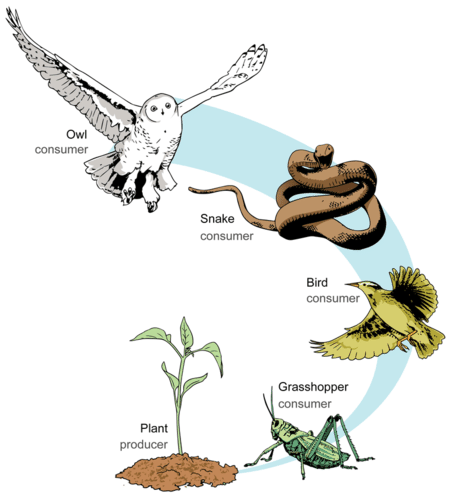
\includegraphics[keepaspectratio]{images/food-chain.png}}

\begin{Shaded}
\begin{Highlighting}[]
\DocumentationTok{\#\# Fraction of basal species}
\NormalTok{FractionOfBasal }\OtherTok{\textless{}{-}} \ControlFlowTok{function}\NormalTok{(M)\{}
\NormalTok{  M\_temp }\OtherTok{\textless{}{-}}\NormalTok{ M;}
  \FunctionTok{diag}\NormalTok{(M\_temp) }\OtherTok{\textless{}{-}} \DecValTok{0}\NormalTok{;}
  
\NormalTok{  b\_sps }\OtherTok{\textless{}{-}} \FunctionTok{sum}\NormalTok{(}\FunctionTok{which}\NormalTok{(}\FunctionTok{InDegree}\NormalTok{(M\_temp) }\SpecialCharTok{==} \DecValTok{0}\NormalTok{) }\SpecialCharTok{\%in\%} \FunctionTok{which}\NormalTok{(}\FunctionTok{OutDegree}\NormalTok{(M\_temp) }\SpecialCharTok{\textgreater{}=} \DecValTok{1}\NormalTok{));}
  
  \FunctionTok{return}\NormalTok{(b\_sps }\SpecialCharTok{/} \FunctionTok{dim}\NormalTok{(M)[}\DecValTok{1}\NormalTok{]);}
\NormalTok{\}}
\end{Highlighting}
\end{Shaded}

Similarly, knowing the fraction of species belonging to intermediate and
top consumer categories can give us information about the degree of
predation pressure and top-down regulation expected in the network, and
its corresponding community, being analysed.

\begin{Shaded}
\begin{Highlighting}[]
\DocumentationTok{\#\# Fraction of top predator species}
\NormalTok{FractionOfTop }\OtherTok{\textless{}{-}} \ControlFlowTok{function}\NormalTok{(M)\{}
\NormalTok{  M\_temp }\OtherTok{\textless{}{-}}\NormalTok{ M;}
  \FunctionTok{diag}\NormalTok{(M\_temp) }\OtherTok{\textless{}{-}} \DecValTok{0}\NormalTok{;}
  
\NormalTok{  t\_sps }\OtherTok{\textless{}{-}} \FunctionTok{sum}\NormalTok{(}\FunctionTok{which}\NormalTok{(}\FunctionTok{InDegree}\NormalTok{(M\_temp) }\SpecialCharTok{\textgreater{}=} \DecValTok{1}\NormalTok{) }\SpecialCharTok{\%in\%} \FunctionTok{which}\NormalTok{(}\FunctionTok{OutDegree}\NormalTok{(M\_temp) }\SpecialCharTok{==} \DecValTok{0}\NormalTok{));}
  
  \FunctionTok{return}\NormalTok{(t\_sps }\SpecialCharTok{/} \FunctionTok{dim}\NormalTok{(M)[}\DecValTok{1}\NormalTok{]);}
\NormalTok{\}}
\end{Highlighting}
\end{Shaded}

\begin{Shaded}
\begin{Highlighting}[]
\DocumentationTok{\#\# Fraction of intermediate consumer species}
\NormalTok{FractionOfIntermediate }\OtherTok{\textless{}{-}} \ControlFlowTok{function}\NormalTok{(M)\{}
\NormalTok{  M\_temp }\OtherTok{\textless{}{-}}\NormalTok{ M;}
  \FunctionTok{diag}\NormalTok{(M\_temp) }\OtherTok{\textless{}{-}} \DecValTok{0}\NormalTok{;}
  
\NormalTok{  i\_sps }\OtherTok{\textless{}{-}} \FunctionTok{sum}\NormalTok{(}\FunctionTok{which}\NormalTok{(}\FunctionTok{InDegree}\NormalTok{(M\_temp) }\SpecialCharTok{\textgreater{}=} \DecValTok{1}\NormalTok{) }\SpecialCharTok{\%in\%} \FunctionTok{which}\NormalTok{(}\FunctionTok{OutDegree}\NormalTok{(M\_temp) }\SpecialCharTok{\textgreater{}=} \DecValTok{1}\NormalTok{));}
  
  \FunctionTok{return}\NormalTok{(i\_sps }\SpecialCharTok{/} \FunctionTok{dim}\NormalTok{(M)[}\DecValTok{1}\NormalTok{]);}
\NormalTok{\}}
\end{Highlighting}
\end{Shaded}

For the Benguela food web we can obtain these properties using the
functions defined above.

\begin{Shaded}
\begin{Highlighting}[]
\FunctionTok{library}\NormalTok{(RCurl)}
\NormalTok{x }\OtherTok{\textless{}{-}} \FunctionTok{getURL}\NormalTok{(}\StringTok{"https://raw.githubusercontent.com/mlurgi/networks\_for\_r/master/datasets/benguela.edgelist"}\NormalTok{)}
\NormalTok{benguela.EL }\OtherTok{\textless{}{-}} \FunctionTok{read.table}\NormalTok{(}\AttributeTok{text =}\NormalTok{ x) }
\NormalTok{benguela.EL }\OtherTok{\textless{}{-}} \FunctionTok{as.matrix}\NormalTok{(benguela.EL)}

\CommentTok{\# Create an adjacency matrix called benguela.AM, containing only zeros}
\NormalTok{benguela.AM }\OtherTok{\textless{}{-}} \FunctionTok{matrix}\NormalTok{(}\DecValTok{0}\NormalTok{, }\FunctionTok{max}\NormalTok{(benguela.EL), }\FunctionTok{max}\NormalTok{(benguela.EL))}

\CommentTok{\# Introduce ones to the matrix to represent interactions between species}
\NormalTok{benguela.AM[benguela.EL] }\OtherTok{\textless{}{-}} \DecValTok{1}

\NormalTok{gen }\OtherTok{\textless{}{-}} \FunctionTok{Generality}\NormalTok{(benguela.AM)}
\NormalTok{vul }\OtherTok{\textless{}{-}} \FunctionTok{Vulnerability}\NormalTok{(benguela.AM)}
\NormalTok{sdgen }\OtherTok{\textless{}{-}} \FunctionTok{SDGenerality}\NormalTok{(benguela.AM)}
\NormalTok{sdvul }\OtherTok{\textless{}{-}} \FunctionTok{SDVulnerability}\NormalTok{(benguela.AM)}
\NormalTok{B }\OtherTok{\textless{}{-}} \FunctionTok{FractionOfBasal}\NormalTok{(benguela.AM)}
\NormalTok{I }\OtherTok{\textless{}{-}} \FunctionTok{FractionOfIntermediate}\NormalTok{(benguela.AM)}
\NormalTok{T }\OtherTok{\textless{}{-}} \FunctionTok{FractionOfTop}\NormalTok{(benguela.AM)}

\FunctionTok{print}\NormalTok{(}\FunctionTok{paste0}\NormalTok{(}\StringTok{\textquotesingle{}Fraction of basal species in Benguela network = \textquotesingle{}}\NormalTok{, }\FunctionTok{round}\NormalTok{(B,}\DecValTok{2}\NormalTok{)))}
\end{Highlighting}
\end{Shaded}

\begin{verbatim}
## [1] "Fraction of basal species in Benguela network = 0.07"
\end{verbatim}

\begin{Shaded}
\begin{Highlighting}[]
\FunctionTok{print}\NormalTok{(}\FunctionTok{paste0}\NormalTok{(}\StringTok{\textquotesingle{}The standard deviation of the vulnerability in the Benguela network is \textquotesingle{}}\NormalTok{, }\FunctionTok{round}\NormalTok{(sdvul,}\DecValTok{2}\NormalTok{)))}
\end{Highlighting}
\end{Shaded}

\begin{verbatim}
## [1] "The standard deviation of the vulnerability in the Benguela network is 0.74"
\end{verbatim}

\subsubsection{Vertical Complexity : Mean Food Chain
Length}\label{vertical-complexity-mean-food-chain-length}

Food chains like those illustrated in the figure above are the exception
rather than the norm in nature. Ecological communities are way more
complex than this, such as the Benguela food web we saw before. You can
imagine a real ecological community as a collection of interconnected
food chains. One way to summarise this complexity is to calculate the
average length of food chains in the network, i.e.~the average number of
links from basal resources to top predators or mean food chaing length.

To be able to quantify this, we need to visit all paths in our network
running from each basal species to each top predator species. This is a
computing intensive task that, for large networks, requires large
computational resources (including long execution times). In graph
theory and network topology, there is considerable research devoted into
how to best count
\href{https://en.wikipedia.org/wiki/Average_path_length}{average paths
in networks}. If you are interested, this is a fascinating area of
research and you can play with functions such as
\href{https://igraph.org/r/doc/distances.html}{distances} on igraph to
find out more.

In food webs, the paths we are interested in are special because they
all start in basal resources and they all stop at top predators. So, the
way in which we should count those paths is a bit different than what
functions such as \texttt{distances} do. Fortunately, there exist
libraries for food web analysis that can help us calculate metrics and
statistics particularly tailored for food webs. One such a package is
\href{http://quicklizard99.github.io/cheddar/}{cheddar}. Cheddar let's
you calculate all of the food web properties we have seen so far and
many more. We will take advantage of cheddar to calculate mean food
chain length. This will also get you familiar with cheddar and you can
explore many more functionalities offered by the package.

Calculating mean food chain length using cheddar:

\begin{Shaded}
\begin{Highlighting}[]
\NormalTok{MeanFoodChainLength }\OtherTok{\textless{}{-}} \ControlFlowTok{function}\NormalTok{(M)\{}
  \FunctionTok{require}\NormalTok{(cheddar)}
\NormalTok{  M }\OtherTok{\textless{}{-}} \FunctionTok{t}\NormalTok{(M)}
\NormalTok{  node }\OtherTok{\textless{}{-}} \DecValTok{1}\SpecialCharTok{:}\FunctionTok{dim}\NormalTok{(M)[}\DecValTok{1}\NormalTok{];}
  \ControlFlowTok{for}\NormalTok{(n }\ControlFlowTok{in} \DecValTok{1}\SpecialCharTok{:}\FunctionTok{length}\NormalTok{(node))\{}
\NormalTok{    node[n] }\OtherTok{\textless{}{-}} \FunctionTok{paste}\NormalTok{(node[n],}\StringTok{\textquotesingle{}{-}\textquotesingle{}}\NormalTok{);}
\NormalTok{  \}}
  
\NormalTok{  pm }\OtherTok{\textless{}{-}} \FunctionTok{matrix}\NormalTok{(M, }\AttributeTok{ncol=}\FunctionTok{dim}\NormalTok{(M)[}\DecValTok{2}\NormalTok{], }\AttributeTok{dimnames=}\FunctionTok{list}\NormalTok{(node, node), }\AttributeTok{byrow=}\ConstantTok{TRUE}\NormalTok{);}
  
  \CommentTok{\# We need to convert our adjacency matrix into a Chedday community object.}
  \CommentTok{\# For this, we yse PredationMatrixToLinks()}
\NormalTok{  community }\OtherTok{\textless{}{-}} \FunctionTok{Community}\NormalTok{(}\AttributeTok{nodes=}\FunctionTok{data.frame}\NormalTok{(}\AttributeTok{node=}\NormalTok{node), }\AttributeTok{trophic.links=}\FunctionTok{PredationMatrixToLinks}\NormalTok{(pm), }\AttributeTok{properties=}\FunctionTok{list}\NormalTok{(}\AttributeTok{title=}\StringTok{\textquotesingle{}Community\textquotesingle{}}\NormalTok{));}
  
  \CommentTok{\# We remove cannibalistic links to avoid entering an infinte loop when calculating path lengths}
\NormalTok{  community }\OtherTok{\textless{}{-}} \FunctionTok{RemoveCannibalisticLinks}\NormalTok{(community, }\AttributeTok{title=}\StringTok{\textquotesingle{}community\textquotesingle{}}\NormalTok{);}
 
\NormalTok{  chain.stats }\OtherTok{\textless{}{-}} \FunctionTok{TrophicChainsStats}\NormalTok{(community)}
\NormalTok{  ch\_lens }\OtherTok{\textless{}{-}}\NormalTok{ (chain.stats}\SpecialCharTok{$}\NormalTok{chain.lengths }\SpecialCharTok{+} \DecValTok{1}\NormalTok{)}
  
  \FunctionTok{return}\NormalTok{(}\FunctionTok{sum}\NormalTok{(ch\_lens)}\SpecialCharTok{/}\FunctionTok{length}\NormalTok{(ch\_lens));}
\NormalTok{\}}

\FunctionTok{print}\NormalTok{(}\FunctionTok{paste0}\NormalTok{(}\StringTok{\textquotesingle{}Mean food chain length in Benguela network = \textquotesingle{}}\NormalTok{, }\FunctionTok{round}\NormalTok{(}\FunctionTok{MeanFoodChainLength}\NormalTok{(benguela.AM),}\DecValTok{2}\NormalTok{)))}
\end{Highlighting}
\end{Shaded}

\begin{verbatim}
## [1] "Mean food chain length in Benguela network = 9.72"
\end{verbatim}

\subsubsection{Degree Distributions}\label{degree-distributions}

Degree distributions constitute a convenient graphical representation of
the probabilities of finding a node in a network possessing a certain
number of links. This property is important because the shape of the
degree distribution of complex networks has been linked to their
robustness to random and targeted attacks to their nodes. In particular,
networks with degree distributions that follow a \emph{power law}, which
are called scale free networks, are robust against random attacks due to
the prevalence of nodes with a small number of links.

Even though the prevalence of truly scale free networks (in the sense of
the degree distributions following exactly a power law) has been
disputed, networks with degree distributions that display a `fat tail'
have been identified in many natural and technological systems from
social networks to the internet. Ecological networks are not an
exception. This suggests that common underlying principles might be
involved in the formation of these networks.

Given its recognised importance and relevance for network persistence we
might be interested in obtaining the degree distribution of our
ecological networks.

To get the degree distribution of the Benguela network we can follow the
instructions below. Since the degree distribution of
\href{https://www.nature.com/articles/nature04927}{ecological networks
has been suggested to generally follow a truncated power law}, we fit
that curve to our data.

\begin{Shaded}
\begin{Highlighting}[]
\CommentTok{\# degrees of the nodes}
\NormalTok{degs }\OtherTok{\textless{}{-}} \FunctionTok{degree}\NormalTok{(benguela.network, }\AttributeTok{mode=}\StringTok{\textquotesingle{}all\textquotesingle{}}\NormalTok{)}

\NormalTok{occur }\OtherTok{=} \FunctionTok{as.vector}\NormalTok{(}\FunctionTok{table}\NormalTok{(degs))}
\NormalTok{occur }\OtherTok{=}\NormalTok{ occur}\SpecialCharTok{/}\FunctionTok{sum}\NormalTok{(occur)}
\NormalTok{p }\OtherTok{=}\NormalTok{ occur}\SpecialCharTok{/}\FunctionTok{sum}\NormalTok{(occur)}
\NormalTok{y }\OtherTok{=} \FunctionTok{rev}\NormalTok{(}\FunctionTok{cumsum}\NormalTok{(}\FunctionTok{rev}\NormalTok{(p)))}
\NormalTok{x }\OtherTok{=} \FunctionTok{as.numeric}\NormalTok{(}\FunctionTok{names}\NormalTok{(}\FunctionTok{table}\NormalTok{(degs)))}

\FunctionTok{plot}\NormalTok{(x, y, }\AttributeTok{log=}\StringTok{"xy"}\NormalTok{, }\AttributeTok{xlab =}\StringTok{\textquotesingle{}log k\textquotesingle{}}\NormalTok{, }\AttributeTok{ylab=}\StringTok{\textquotesingle{}log Pc(k)\textquotesingle{}}\NormalTok{, }\AttributeTok{type=}\StringTok{\textquotesingle{}p\textquotesingle{}}\NormalTok{, }\AttributeTok{col=}\StringTok{\textquotesingle{}black\textquotesingle{}}\NormalTok{, }\AttributeTok{pch=}\DecValTok{16}\NormalTok{)}

\FunctionTok{box}\NormalTok{(}\AttributeTok{lwd=}\FloatTok{1.5}\NormalTok{)}

\CommentTok{\# and we fit a truncated power law to the data}
\NormalTok{temp }\OtherTok{\textless{}{-}} \FunctionTok{data.frame}\NormalTok{(x,y)}
\NormalTok{mod1 }\OtherTok{\textless{}{-}} \FunctionTok{nls}\NormalTok{(y }\SpecialCharTok{\textasciitilde{}}\NormalTok{ (x}\SpecialCharTok{\^{}{-}}\NormalTok{a}\SpecialCharTok{*}\FunctionTok{exp}\NormalTok{(}\SpecialCharTok{{-}}\NormalTok{x}\SpecialCharTok{/}\NormalTok{b)), }\AttributeTok{data =}\NormalTok{ temp, }\AttributeTok{start =} \FunctionTok{list}\NormalTok{(}\AttributeTok{a =} \DecValTok{1}\NormalTok{, }\AttributeTok{b =} \DecValTok{1}\NormalTok{))}

\CommentTok{\# add fitted curve}
\FunctionTok{lines}\NormalTok{(temp}\SpecialCharTok{$}\NormalTok{x, }\FunctionTok{predict}\NormalTok{(mod1, }\FunctionTok{list}\NormalTok{(}\AttributeTok{x =}\NormalTok{ temp}\SpecialCharTok{$}\NormalTok{x)), }\AttributeTok{col=}\StringTok{\textquotesingle{}red\textquotesingle{}}\NormalTok{)}
\end{Highlighting}
\end{Shaded}

\pandocbounded{\includegraphics[keepaspectratio]{networks-session_files/figure-latex/unnamed-chunk-26-1.pdf}}

\subsection{Dynamics in networks: An example from an extinction
experiment}\label{dynamics-in-networks-an-example-from-an-extinction-experiment}

The development of predictive frameworks for complex ecosystems relies
on mathematical and computational tools. One approach is the use of
ordinary differential equations (ODEs) to simulate network dynamics.
\textbf{The history of dynamical modelling of this kind in ecology began
back in the 1920's with the works by Alfred J. Lotka and Vito Volterra}.
Lotka and Volterra developed independently a similar set of two coupled
differential equations to study the dynamics of biological systems in
general (Lotka) and the effect of restricting fisheries for predatory
fish in the Adriatic Sea (Volterra). These equations have become to be
known as the Lotka-Volterra model, and it is one of the most used
mathematical models in ecology to study the temporal dynamics of
predator and prey populations.

\includegraphics[width=2.08333in,height=\textheight,keepaspectratio]{images/lotka-volterra.png}

\[
\frac{dx}{dt} = \alpha x - \beta xy
\] \[
\frac{dy}{dt} = \delta xy - \gamma y
\]

where \(x\) and \(y\) are the abundances of prey and predator
respectively, and \(\alpha, \beta,\delta,\) and \(\gamma\) are the model
parameters that control the intrinsic growth rate of the prey species,
the prey loss due to predatory attack, the gain of the predator when
consuming prey (which includes the efficiency of the energy transfer
across trophic levels), and the death rate of predators, respectively.

Here, our focus is on how to use these coupled equations to simulate
dynamics of many species in a network with a given pattern of
connectivity that determines these interactions. In the general case of
the equations above, when extended to many species we can write the
equations in a comprised format thus:

\[
\frac{dN_i}{dt} = N_i \left(r_i + \sum_{j=1}^{n} \alpha_{ij}N_j \right) , i = 1 ... n
\]

where \(N_i\) are the abundance of species \(i\), \(r_i\) is the
intrinsic growth (or death) rate of species \(i\) (positive for
intrinsically growing basal species, and negative for consumers), and
the \(\alpha_{ij}\)'s represent the interaction coefficients between
species. If we further compact all interaction coefficients into
matricial form, and represent abundances and growth rates as vectors we
obtain:

\[
\frac{dN}{dt} = N * (r+AN)
\]

To solve a system of ODEs like the one above numerically, we can use
programming libraries available that perform the numerical integration
for us. These are available across many platforms, although here we
stick to R.

\begin{Shaded}
\begin{Highlighting}[]
\CommentTok{\# loading required libraries}
\FunctionTok{require}\NormalTok{(deSolve)}
\FunctionTok{require}\NormalTok{(igraph)}

\CommentTok{\# Defining the generalised Lotka{-}Volterra model}
\CommentTok{\# Taken from Allesina\textquotesingle{}s code (see link in the text)}
\NormalTok{generalised.LV }\OtherTok{\textless{}{-}} \ControlFlowTok{function}\NormalTok{(t, x, parameters)\{}
  \FunctionTok{with}\NormalTok{(}\FunctionTok{as.list}\NormalTok{(}\FunctionTok{c}\NormalTok{(x, parameters)), \{}
\NormalTok{    x[x }\SpecialCharTok{\textless{}} \DecValTok{10}\SpecialCharTok{\^{}{-}}\DecValTok{8}\NormalTok{] }\OtherTok{\textless{}{-}} \DecValTok{0} \CommentTok{\# to avoid prevent numerical problems}
\NormalTok{    dxdt }\OtherTok{\textless{}{-}}\NormalTok{ x }\SpecialCharTok{*}\NormalTok{ (b }\SpecialCharTok{+}\NormalTok{ A }\SpecialCharTok{\%*\%}\NormalTok{ x)}
    \FunctionTok{list}\NormalTok{(dxdt)}
\NormalTok{  \})}
\NormalTok{\}}

\CommentTok{\# This function is for performing simulation experiments}
\NormalTok{run\_community\_dynamics }\OtherTok{\textless{}{-}} \ControlFlowTok{function}\NormalTok{(A, b, }\AttributeTok{init\_abs=}\ConstantTok{NULL}\NormalTok{)\{}
\NormalTok{  nb\_species }\OtherTok{\textless{}{-}} \FunctionTok{dim}\NormalTok{(A)[}\DecValTok{1}\NormalTok{]           }\CommentTok{\# the number of species}
\NormalTok{  nb\_pos }\OtherTok{\textless{}{-}} \FunctionTok{length}\NormalTok{(}\FunctionTok{which}\NormalTok{(A }\SpecialCharTok{\textgreater{}} \DecValTok{0}\NormalTok{))        }\CommentTok{\# the number of + interactions}
\NormalTok{  nb\_neg }\OtherTok{\textless{}{-}} \FunctionTok{length}\NormalTok{(}\FunctionTok{which}\NormalTok{(A }\SpecialCharTok{\textless{}} \DecValTok{0}\NormalTok{))        }\CommentTok{\# the number of {-} interactions}
\NormalTok{  pos }\OtherTok{\textless{}{-}} \FunctionTok{runif}\NormalTok{(nb\_pos, }\DecValTok{0}\NormalTok{, }\FloatTok{0.05}\NormalTok{) }\CommentTok{\# uniform distribution positive effects}
\NormalTok{  neg }\OtherTok{\textless{}{-}} \FunctionTok{runif}\NormalTok{(nb\_neg, }\SpecialCharTok{{-}}\FloatTok{0.5}\NormalTok{, }\DecValTok{0}\NormalTok{) }\CommentTok{\# uniform distribution negative effects}
  
\NormalTok{  A[A}\SpecialCharTok{\textless{}}\DecValTok{0}\NormalTok{] }\OtherTok{\textless{}{-}}\NormalTok{ neg}
\NormalTok{  A[A}\SpecialCharTok{\textgreater{}}\DecValTok{0}\NormalTok{] }\OtherTok{\textless{}{-}}\NormalTok{ pos}
  
  \CommentTok{\# initial abundances from a uniform distribution between 0 and 1}
  \ControlFlowTok{if}\NormalTok{(}\FunctionTok{is.null}\NormalTok{(init\_abs))}
\NormalTok{    N0 }\OtherTok{\textless{}{-}} \FunctionTok{runif}\NormalTok{(nb\_species, }\FloatTok{0.01}\NormalTok{, .}\DecValTok{1}\NormalTok{)}
  \ControlFlowTok{else}
\NormalTok{    N0 }\OtherTok{\textless{}{-}}\NormalTok{ init\_abs}
  
  \CommentTok{\# definition of time}
\NormalTok{  t.values }\OtherTok{\textless{}{-}} \FunctionTok{seq}\NormalTok{(}\DecValTok{0}\NormalTok{, }\DecValTok{500}\NormalTok{, }\AttributeTok{by=}\FloatTok{0.01}\NormalTok{)}
  
  \CommentTok{\# here we set the values of the parameters that the equations take}
\NormalTok{  params }\OtherTok{\textless{}{-}} \FunctionTok{list}\NormalTok{(}\AttributeTok{b =}\NormalTok{ b, }\AttributeTok{A =}\NormalTok{ A)}
  
  \CommentTok{\# solve numerically}
\NormalTok{  glv.out }\OtherTok{\textless{}{-}} \FunctionTok{ode}\NormalTok{(}\AttributeTok{y =}\NormalTok{ N0, }\AttributeTok{times =}\NormalTok{ t.values, }\AttributeTok{func =}\NormalTok{ generalised.LV, }\AttributeTok{parms =}\NormalTok{ params)}
  \FunctionTok{return}\NormalTok{(glv.out)}
\NormalTok{\}}

\FunctionTok{set.seed}\NormalTok{(}\DecValTok{924}\NormalTok{)               }\CommentTok{\# setting seed for reproducibility}

\CommentTok{\# We define the interaction matrix / network A}
\NormalTok{A }\OtherTok{\textless{}{-}} \FunctionTok{matrix}\NormalTok{(}\FunctionTok{c}\NormalTok{(}\SpecialCharTok{{-}}\DecValTok{1}\NormalTok{,}\SpecialCharTok{{-}}\DecValTok{1}\NormalTok{,}\DecValTok{0}\NormalTok{,}\DecValTok{0}\NormalTok{,}\SpecialCharTok{{-}}\DecValTok{1}\NormalTok{,}\DecValTok{0}\NormalTok{,}
              \DecValTok{1}\NormalTok{,}\DecValTok{0}\NormalTok{,}\SpecialCharTok{{-}}\DecValTok{1}\NormalTok{,}\DecValTok{1}\NormalTok{,}\DecValTok{0}\NormalTok{,}\DecValTok{0}\NormalTok{,}
              \DecValTok{0}\NormalTok{,}\DecValTok{1}\NormalTok{,}\DecValTok{0}\NormalTok{,}\DecValTok{0}\NormalTok{,}\DecValTok{0}\NormalTok{,}\DecValTok{0}\NormalTok{,}
              \DecValTok{0}\NormalTok{,}\SpecialCharTok{{-}}\DecValTok{1}\NormalTok{,}\DecValTok{0}\NormalTok{,}\SpecialCharTok{{-}}\DecValTok{1}\NormalTok{,}\SpecialCharTok{{-}}\DecValTok{1}\NormalTok{,}\DecValTok{0}\NormalTok{,}
              \DecValTok{1}\NormalTok{,}\DecValTok{0}\NormalTok{,}\DecValTok{0}\NormalTok{,}\DecValTok{1}\NormalTok{,}\DecValTok{0}\NormalTok{,}\SpecialCharTok{{-}}\DecValTok{1}\NormalTok{,}
              \DecValTok{0}\NormalTok{,}\DecValTok{0}\NormalTok{,}\DecValTok{0}\NormalTok{,}\DecValTok{0}\NormalTok{,}\DecValTok{1}\NormalTok{,}\DecValTok{0}\NormalTok{), }\DecValTok{6}\NormalTok{, }\DecValTok{6}\NormalTok{, }\AttributeTok{byrow =} \ConstantTok{TRUE}\NormalTok{)}


\CommentTok{\# here we run the simulations using the network above}
\NormalTok{b }\OtherTok{\textless{}{-}} \FunctionTok{c}\NormalTok{(}\DecValTok{1}\NormalTok{, }\SpecialCharTok{{-}}\FloatTok{0.02}\NormalTok{, }\SpecialCharTok{{-}}\FloatTok{0.02}\NormalTok{, }\DecValTok{1}\NormalTok{, }\SpecialCharTok{{-}}\FloatTok{0.02}\NormalTok{, }\SpecialCharTok{{-}}\FloatTok{0.02}\NormalTok{)}
\NormalTok{output }\OtherTok{\textless{}{-}} \FunctionTok{run\_community\_dynamics}\NormalTok{(A, b)}

\CommentTok{\# And we plot the results...}
\DocumentationTok{\#\#\#\#\# Stuff for layouting the network \#\#\#\#\#\#}
\DocumentationTok{\#\# This is just layouting instructions for the network to look pretty. Don’t waste too much time in this}
\NormalTok{food\_web\_layout }\OtherTok{\textless{}{-}} \FunctionTok{matrix}\NormalTok{(}\FunctionTok{c}\NormalTok{( }\SpecialCharTok{{-}}\FloatTok{1.37859603}\NormalTok{, }\SpecialCharTok{{-}}\FloatTok{3.5772072}\NormalTok{,}
                             \SpecialCharTok{{-}}\FloatTok{1.37859603}\NormalTok{, }\SpecialCharTok{{-}}\FloatTok{0.0374094}\NormalTok{,}
                             \SpecialCharTok{{-}}\FloatTok{1.37859603}\NormalTok{,  }\FloatTok{3.5772072}\NormalTok{,}
                             \FloatTok{1.37859603}\NormalTok{, }\SpecialCharTok{{-}}\FloatTok{3.5772072}\NormalTok{,}
                             \FloatTok{1.37859603}\NormalTok{, }\SpecialCharTok{{-}}\FloatTok{0.0374094}\NormalTok{,}
                             \FloatTok{1.37859603}\NormalTok{,   }\FloatTok{3.5772072}\NormalTok{), }\DecValTok{6}\NormalTok{, }\DecValTok{2}\NormalTok{, }\AttributeTok{byrow=}\ConstantTok{TRUE}\NormalTok{)}

\CommentTok{\# This is to ensure we plot the network as we want to see it}
\NormalTok{A\_plot }\OtherTok{\textless{}{-}} \FunctionTok{t}\NormalTok{(A)}
\NormalTok{A\_plot[A\_plot }\SpecialCharTok{\textless{}} \DecValTok{0}\NormalTok{] }\OtherTok{\textless{}{-}} \DecValTok{0}
\FunctionTok{diag}\NormalTok{(A\_plot) }\OtherTok{\textless{}{-}} \DecValTok{0}
\NormalTok{g }\OtherTok{\textless{}{-}} \FunctionTok{graph\_from\_adjacency\_matrix}\NormalTok{(A\_plot)}

\CommentTok{\# defining the colours for the figures}
\NormalTok{colours }\OtherTok{\textless{}{-}} \FunctionTok{c}\NormalTok{(}\StringTok{\textquotesingle{}red2\textquotesingle{}}\NormalTok{, }\StringTok{\textquotesingle{}black\textquotesingle{}}\NormalTok{, }\StringTok{\textquotesingle{}darkolivegreen3\textquotesingle{}}\NormalTok{, }\StringTok{\textquotesingle{}darkcyan\textquotesingle{}}\NormalTok{, }\StringTok{\textquotesingle{}darkorchid1\textquotesingle{}}\NormalTok{, }\StringTok{\textquotesingle{}blue\textquotesingle{}}\NormalTok{)}
\DocumentationTok{\#\#\#\#\#\#\#\#\#\#\#\#\#\#\#\#\#\#}


\FunctionTok{par}\NormalTok{(}\AttributeTok{fig=}\FunctionTok{c}\NormalTok{(}\DecValTok{0}\NormalTok{,}\DecValTok{10}\NormalTok{,}\DecValTok{0}\NormalTok{,}\DecValTok{10}\NormalTok{)}\SpecialCharTok{/}\DecValTok{10}\NormalTok{)}
\FunctionTok{par}\NormalTok{(}\AttributeTok{mar=}\FunctionTok{c}\NormalTok{(}\DecValTok{5}\NormalTok{,}\DecValTok{5}\NormalTok{,}\DecValTok{0}\NormalTok{,}\DecValTok{0}\NormalTok{))}
\FunctionTok{matplot}\NormalTok{((output[,}\FunctionTok{c}\NormalTok{(}\DecValTok{2}\SpecialCharTok{:}\DecValTok{7}\NormalTok{)]), }\AttributeTok{type =} \StringTok{\textquotesingle{}l\textquotesingle{}}\NormalTok{, }\AttributeTok{lty =} \DecValTok{1}\NormalTok{, }\AttributeTok{lwd =} \DecValTok{2}\NormalTok{, }\AttributeTok{ylab=}\StringTok{\textquotesingle{}Abudance\textquotesingle{}}\NormalTok{, }\AttributeTok{xlab=}\StringTok{\textquotesingle{}Time\textquotesingle{}}\NormalTok{,}\AttributeTok{col=}\NormalTok{ colours, }\AttributeTok{ylim=}\FunctionTok{c}\NormalTok{(}\DecValTok{0}\NormalTok{,}\DecValTok{5}\NormalTok{))}
\end{Highlighting}
\end{Shaded}

\pandocbounded{\includegraphics[keepaspectratio]{networks-session_files/figure-latex/generalised-lv-1.pdf}}

\begin{Shaded}
\begin{Highlighting}[]
\FunctionTok{par}\NormalTok{(}\AttributeTok{fig=}\FunctionTok{c}\NormalTok{(}\FloatTok{6.5}\NormalTok{,}\FloatTok{9.5}\NormalTok{,}\FloatTok{5.5}\NormalTok{,}\DecValTok{10}\NormalTok{)}\SpecialCharTok{/}\DecValTok{10}\NormalTok{)}
\FunctionTok{par}\NormalTok{(}\AttributeTok{new=}\NormalTok{T, }\AttributeTok{mar=}\FunctionTok{c}\NormalTok{(}\DecValTok{0}\NormalTok{,}\DecValTok{0}\NormalTok{,}\DecValTok{0}\NormalTok{,}\DecValTok{1}\NormalTok{))}
\FunctionTok{plot}\NormalTok{(g, }\AttributeTok{layout=}\NormalTok{food\_web\_layout, }\AttributeTok{vertex.color =}\NormalTok{ colours, }\AttributeTok{vertex.label.color=}\StringTok{\textquotesingle{}white\textquotesingle{}}\NormalTok{, }\AttributeTok{vertex.size=}\DecValTok{25}\NormalTok{, }\AttributeTok{vertex.label.cex=}\DecValTok{1}\NormalTok{)}
\end{Highlighting}
\end{Shaded}

\pandocbounded{\includegraphics[keepaspectratio]{networks-session_files/figure-latex/generalised-lv-2.pdf}}

On models like this we can then remove or add species and assess the
effect that those perturbations have on the resulting community. For
example, removing species 4 from the network above results in more
stable populations of consumers (i.e.~less drastic fluctuations) and
reduced abundance of top predator species (compare abundances of top
species 3 across plots).

\begin{Shaded}
\begin{Highlighting}[]
\CommentTok{\# We remove species 4 from the system and have to redefine the network and the parameter vectors}
\CommentTok{\# We extract initial abundances from the previous outcome}
\NormalTok{cur\_abs }\OtherTok{\textless{}{-}}\NormalTok{ output[}\FunctionTok{dim}\NormalTok{(output)[}\DecValTok{1}\NormalTok{], }\SpecialCharTok{{-}}\FunctionTok{c}\NormalTok{(}\DecValTok{1}\NormalTok{,}\DecValTok{5}\NormalTok{)]}

\NormalTok{A\_no\_4 }\OtherTok{\textless{}{-}} \FunctionTok{matrix}\NormalTok{(}\FunctionTok{c}\NormalTok{(}\SpecialCharTok{{-}}\DecValTok{1}\NormalTok{,}\SpecialCharTok{{-}}\DecValTok{1}\NormalTok{,}\DecValTok{0}\NormalTok{,}\SpecialCharTok{{-}}\DecValTok{1}\NormalTok{,}\DecValTok{0}\NormalTok{,}
                   \DecValTok{1}\NormalTok{,}\DecValTok{0}\NormalTok{,}\SpecialCharTok{{-}}\DecValTok{1}\NormalTok{,}\DecValTok{0}\NormalTok{,}\DecValTok{0}\NormalTok{,}
                   \DecValTok{0}\NormalTok{,}\DecValTok{1}\NormalTok{,}\DecValTok{0}\NormalTok{,}\DecValTok{0}\NormalTok{,}\DecValTok{0}\NormalTok{,}
                   \DecValTok{1}\NormalTok{,}\DecValTok{0}\NormalTok{,}\DecValTok{0}\NormalTok{,}\DecValTok{0}\NormalTok{,}\SpecialCharTok{{-}}\DecValTok{1}\NormalTok{,}
                   \DecValTok{0}\NormalTok{,}\DecValTok{0}\NormalTok{,}\DecValTok{0}\NormalTok{,}\DecValTok{1}\NormalTok{,}\DecValTok{0}\NormalTok{), }\DecValTok{5}\NormalTok{, }\DecValTok{5}\NormalTok{, }\AttributeTok{byrow =} \ConstantTok{TRUE}\NormalTok{)}


\FunctionTok{set.seed}\NormalTok{(}\DecValTok{924}\NormalTok{)               }\CommentTok{\# setting seed}
\NormalTok{b }\OtherTok{\textless{}{-}} \FunctionTok{c}\NormalTok{(}\DecValTok{1}\NormalTok{, }\SpecialCharTok{{-}}\FloatTok{0.02}\NormalTok{, }\SpecialCharTok{{-}}\FloatTok{0.02}\NormalTok{, }\SpecialCharTok{{-}}\FloatTok{0.02}\NormalTok{, }\SpecialCharTok{{-}}\FloatTok{0.02}\NormalTok{)}
\NormalTok{output\_extinction }\OtherTok{\textless{}{-}} \FunctionTok{run\_community\_dynamics}\NormalTok{(A\_no\_4, b, cur\_abs)}

\CommentTok{\# plotting the results}
\CommentTok{\# new network (without species 4) requires new layout}
\NormalTok{food\_web\_layout\_2 }\OtherTok{\textless{}{-}} \FunctionTok{matrix}\NormalTok{(}\FunctionTok{c}\NormalTok{( }\SpecialCharTok{{-}}\FloatTok{1.37859603}\NormalTok{, }\SpecialCharTok{{-}}\FloatTok{3.5772072}\NormalTok{,}
                               \SpecialCharTok{{-}}\FloatTok{1.37859603}\NormalTok{, }\SpecialCharTok{{-}}\FloatTok{0.0374094}\NormalTok{,}
                               \SpecialCharTok{{-}}\FloatTok{1.37859603}\NormalTok{,  }\FloatTok{3.5772072}\NormalTok{,}
                               \FloatTok{1.37859603}\NormalTok{, }\SpecialCharTok{{-}}\FloatTok{0.0374094}\NormalTok{,}
                               \FloatTok{1.37859603}\NormalTok{,   }\FloatTok{3.5772072}\NormalTok{), }\DecValTok{5}\NormalTok{, }\DecValTok{2}\NormalTok{, }\AttributeTok{byrow=}\ConstantTok{TRUE}\NormalTok{)}

\CommentTok{\# again just to plot the new network}
\NormalTok{A\_plot }\OtherTok{\textless{}{-}} \FunctionTok{t}\NormalTok{(A\_no\_4)}
\NormalTok{A\_plot[A\_plot }\SpecialCharTok{\textless{}} \DecValTok{0}\NormalTok{] }\OtherTok{\textless{}{-}} \DecValTok{0}
\FunctionTok{diag}\NormalTok{(A\_plot) }\OtherTok{\textless{}{-}} \DecValTok{0}
\NormalTok{g }\OtherTok{\textless{}{-}} \FunctionTok{graph\_from\_adjacency\_matrix}\NormalTok{(A\_plot)}

\FunctionTok{par}\NormalTok{(}\AttributeTok{fig=}\FunctionTok{c}\NormalTok{(}\DecValTok{0}\NormalTok{,}\DecValTok{10}\NormalTok{,}\DecValTok{0}\NormalTok{,}\DecValTok{10}\NormalTok{)}\SpecialCharTok{/}\DecValTok{10}\NormalTok{)}
\FunctionTok{par}\NormalTok{(}\AttributeTok{mar=}\FunctionTok{c}\NormalTok{(}\DecValTok{5}\NormalTok{,}\DecValTok{5}\NormalTok{,}\DecValTok{0}\NormalTok{,}\DecValTok{0}\NormalTok{))}
\FunctionTok{matplot}\NormalTok{((output\_extinction[,}\FunctionTok{c}\NormalTok{(}\DecValTok{2}\SpecialCharTok{:}\DecValTok{6}\NormalTok{)]), }\AttributeTok{type =} \StringTok{\textquotesingle{}l\textquotesingle{}}\NormalTok{, }\AttributeTok{lty =} \DecValTok{1}\NormalTok{, }\AttributeTok{lwd =} \DecValTok{2}\NormalTok{, }\AttributeTok{ylab=}\StringTok{\textquotesingle{}Abudance\textquotesingle{}}\NormalTok{, }\AttributeTok{xlab=}\StringTok{\textquotesingle{}Time\textquotesingle{}}\NormalTok{, }\AttributeTok{col=}\NormalTok{colours[}\SpecialCharTok{{-}}\DecValTok{4}\NormalTok{])}
\end{Highlighting}
\end{Shaded}

\pandocbounded{\includegraphics[keepaspectratio]{networks-session_files/figure-latex/extinction-1.pdf}}

\begin{Shaded}
\begin{Highlighting}[]
\FunctionTok{par}\NormalTok{(}\AttributeTok{fig=}\FunctionTok{c}\NormalTok{(}\FloatTok{6.5}\NormalTok{,}\FloatTok{9.5}\NormalTok{,}\FloatTok{5.5}\NormalTok{,}\DecValTok{10}\NormalTok{)}\SpecialCharTok{/}\DecValTok{10}\NormalTok{)}
\FunctionTok{par}\NormalTok{(}\AttributeTok{new=}\NormalTok{T, }\AttributeTok{mar=}\FunctionTok{c}\NormalTok{(}\DecValTok{0}\NormalTok{,}\DecValTok{0}\NormalTok{,}\DecValTok{0}\NormalTok{,}\DecValTok{1}\NormalTok{))}

\FunctionTok{plot}\NormalTok{(g, }\AttributeTok{layout=}\NormalTok{food\_web\_layout\_2, }\AttributeTok{vertex.color =}\NormalTok{ colours[}\SpecialCharTok{{-}}\DecValTok{4}\NormalTok{], }\AttributeTok{vertex.label.color=}\StringTok{\textquotesingle{}white\textquotesingle{}}\NormalTok{, }\AttributeTok{vertex.size=}\DecValTok{25}\NormalTok{, }\AttributeTok{vertex.label.cex=}\DecValTok{1}\NormalTok{, }\AttributeTok{vertex.label=}\FunctionTok{c}\NormalTok{(}\DecValTok{1}\SpecialCharTok{:}\DecValTok{3}\NormalTok{, }\DecValTok{5}\NormalTok{,}\DecValTok{6}\NormalTok{))}
\end{Highlighting}
\end{Shaded}

\pandocbounded{\includegraphics[keepaspectratio]{networks-session_files/figure-latex/extinction-2.pdf}}

This example illustrates the use of dynamical models of networks in
community ecology and how we can used them to answer research questions
in ecology.

\subsection{References}\label{references}

Bascompte, J and Jordano P (2007) Plant-Animal Mutualistic Networks: The
Architecture of Biodiversity. \textbf{\emph{Annual Review of Ecology,
Evolution, and Systematics}} 38(1), 567-593.

Montoya, J., Pimm, S. \& Solé, R. (2006) Ecological networks and their
fragility. \textbf{\emph{Nature}}, 442, 259--264.

Newman, M. E. J. (2003) The Structure and Function of Complex Networks.
\textbf{\emph{SIAM Rev.}}, 45(2), 167--256.

Ollerton, J. et al.~(2007) Finding NEMO: nestedness engendered by
mutualistic organization in anemonefish and their hosts.
\textbf{Proceedings of the Royal Society B}, 274, 591-598.

\end{document}
